\documentclass[a4paper, 12pt]{report}
\usepackage[utf8]{vietnam}
\usepackage{amsmath}
\usepackage{amsfonts}
\usepackage{amssymb}
\usepackage{amsthm}
\usepackage{fancyhdr}
\usepackage{mathrsfs}
\usepackage[left=3.5cm,right=2cm,top=3.5cm,bottom=3cm]{geometry}
\usepackage{graphicx}
\usepackage{tikz}
\usepackage{float}
\usepackage{pdfpages}

\usepackage{eufrak}
\usepackage{listings}
\usepackage{tabu}
\renewcommand{\baselinestretch}{1.5}
\setlength{\parindent}{0pt}
\pagestyle{plain}
%\documentclass{article}
%\usepackage{indentfirst}
\usepackage{graphicx}
\usepackage{enumitem}

\usepackage[vietnamese=nohyphenation]{hyphsubst}
\usepackage[vietnamese]{babel}
%\setlength{\parindent}{1cm} % Default is 15pt.

\usepackage{titlesec}
\usepackage{subcaption}

\titleformat*{\section}{\LARGE\bfseries}
\titleformat*{\subsection}{\Large\bfseries}
\titleformat*{\subsubsection}{\large\bfseries}
\titleformat*{\paragraph}{\large\bfseries}
\titleformat*{\subparagraph}{\large\bfseries}

%\newtheorem{theorem}{Định lý}[section]

%\newtheorem*{theorem}{Định lý}[section]
%\newtheorem{theorem}{Theorem}
\usepackage{amsthm}

\newtheorem*{theorem}{Định lý } %without numbering
\newtheorem*{corollary}{Hệ quả } %without numbering
\newtheorem{theoremnum}{Định lý } %without numbering

% \newtheorem{theorem}{Theorem}  %with numberring

\newtheorem{Proposition}{Mệnh đề } %without numbering
\newtheorem*{Propositionproof}{Chứng minh mệnh đề 1: } %without numbering
\newtheorem{claim}{Khẳng định}
\pagestyle{fancy}
\fancyhead{}
\fancyhead[L]{}
\fancyhead[R]{\itshape Đồ án tốt nghiệp 20201}

\fancyfoot{}
\fancyfoot[L]{\itshape Thực hiện: Lai Đức Thắng}
\fancyfoot[R]{Toán Tin K61}
%\lfoot{\textit{Lai Đức Thắng}}
%
%\rfoot{\textit{Toán Tin K61}}

\renewcommand{\footrulewidth}{1,2pt}



\begin{document}



	\begin{titlepage} % Đây là trang bìa


			\begin{center}
				
				{\large\bf TRƯỜNG ĐẠI HỌC BÁCH KHOA HÀ NỘI}\\
				
				{\large\bf VIỆN TOÁN ỨNG DỤNG VÀ TIN HỌC} \\
				
				{———————o0o——————–}
				\vskip 1cm
%			\includegraphics[scale=0.3]{Logo_Hust}
				\begin{center}
     				
\includegraphics[scale=.85]{Images/biaDA.png}
				\end{center}
				\vskip 1cm
				
%				{\Large\bf \textbf{PHƯƠNG PHÁP\\ 
%						PHÂN TÍCH THÀNH PHẦN CHÍNH\\
%						(Principal Component Analysis - PCA )
%				}}

				{\Large\bf \textbf{HỌC SÂU
						VÀ ỨNG DỤNG TRONG\\ BÀI TOÁN ĐẾM CÂY\\
				}}
				\vskip 1cm
				{\bf ĐỒ ÁN TỐT NGHIỆP ĐẠI HỌC}
				
				
				{\bf {\it Chuyên ngành:} TOÁN TIN}\\
%				{\bf {\it Chuyên sâu:} }Xác suất rời rạc
				
				\vskip 1cm
				
				\begin{tabular}{r l}
					
					Giảng viên hướng dẫn:&{\bf TS.  LÊ HẢI HÀ  }\\[0.5cm]
					
					Họ và tên sinh viên:&{\bf LAI ĐỨC THẮNG}\\[0.5cm]
					
					Số hiệu sinh viên:&{\bf 20163830}\\[0.5cm]
					Lớp:&{\bf Toán Tin K61}
					
				\end{tabular}
				
				\vfill
				
				{\bf HÀ NỘI - 2020}
				
			\end{center}
			
	\end{titlepage}

\tableofcontents{}

\chapter*{Danh mục từ viết tắt}
\addcontentsline{toc}{chapter}{Danh mục từ viết tắt}


\chapter*{Danh sách hình vẽ}
\addcontentsline{toc}{chapter}{Danh sách hình vẽ}

\chapter*{Lời cảm ơn}
\addcontentsline{toc}{chapter}{Lời cảm ơn}	

\chapter*{Lời mở đầu}
\addcontentsline{toc}{chapter}{Lời mở đầu}
Việc sản xuất và phân phối loại cây trồng có giá trị kinh tế này đòi hỏi phải có sự giám sát thường xuyên đối với theo chu kì và theo mùa vụ. Đây là một nhiệm vụ quan trọng đối với việc quản lý tài nguyên, rừng. Để đáp ứng nhu cầu ngày càng tăng của thế giới và sản lượng nông nghiệp tiêu dùng, năng suất cây trồng phải được ước tính. Việc phát hiện, thu thập thủ công dữ liệu cây trồng để lưu trữ hồ sơ trên một diễn tích đất lớn là không khả thi đối với con người, gây tốn kém tiền bạc và dễ bị ảnh hưởng bởi lỗi của con người
Việc phát hiện cây trên một diện tích lớn sẽ giúp doanh nghiệp giảm bớt sự phụ thuộc vào con người và chi phí, dễ dàng quản lý và lên kế hoạch kịp thời cho sản xuất. Trong vài năm trở lại đây, lĩnh vực học sâu và xử lý ảnh đang nhận được nhiều sự quan tâm, áp dụng trong nhiều lĩnh vực khoa học khác nhau. Trong báo cáo đồ án này, em xin giới thiệu một giải phát phát hiện cây trong các bức ảnh viễn thám dựa trên mô hình học sâu. Nội dung của đồ án gồm có phần mở đầu, 4 chương, phần kết luận, tài liệu tham khảo:
\begin{itemize}
	\item \textbf{Chương 1: }
	
	\item \textbf{Chương 2: }

	\item \textbf{Chương 3: }

\end{itemize}

\chapter{Lý thuyết về hệ thống thông tin địa lý và tiền xử lý ảnh viễn thám}

\section{Hệ thống thông tin địa lý}

\section{Ảnh viễn thám và quá trình tiền xử lý}




\chapter{Lý thuyết học sâu và bài toán nhận diện vật thể}
Deep Learning là một kỹ thuật Machine Learning mà ở đó huấn luyện máy tính giống như cách thức tự nhiên của con người: Học qua các ví dụ. Những năm gần đây, Deep learning đã mang đến nhiều bất ngờ trên quy mô toàn cầu và dẫn đường cho những tiến triển nhanh chóng trong nhiều lĩnh vực khác nhau như thị giác máy tính, xử lý ngôn ngữ tự nhiên (natural language processing), nhận dạng giọng nói tự động (automatic speech recognition), học tăng cường (reinforcement learning), và mô hình hoá thống kê (statistical modeling). Với những tiến bộ này, chúng ta bây giờ có thể xây dựng xe tự lái với mức độ tự động ngày càng cao (nhưng chưa nhiều tới mức như vài công ty đang tuyên bố), xây dựng các hệ thống giúp trả lời thư tự động khi con người ngập trong núi email, hay lập trình phần mềm chơi cờ vây có thể thắng cả nhà vô địch thế giới, một kỳ tích từng được xem là không thể đạt được trong nhiều thập kỷ tới. Những công cụ này đã và đang gây ảnh hưởng rộng rãi tới các ngành công nghiệp và đời sống xã hội, thay đổi cách tạo ra các bộ phim, cách chẩn đoán bệnh và đóng một vài trò ngày càng tăng trong các ngành khoa học cơ bản – từ vật lý thiên văn tới sinh học.\par
Với Deep Learning, một mô hình máy tính học cách thực hiện một công việc phân loại (classification) trực tiếp từ các hình ảnh, chữ viết (text) hoặc âm thanh. Các mô hình (models) Deep Learning có thể đạt được độ chính xác cao, đôi khi còn hơn cả con người. Các mô hình được huấn luyện bởi việc sử dụng một tập bao gồm bộ dữ liệu được gán nhãn và các kiến trúc mạng neural gồm nhiều lớp (layer). \par
\begin{figure}[!h]
	\centering
	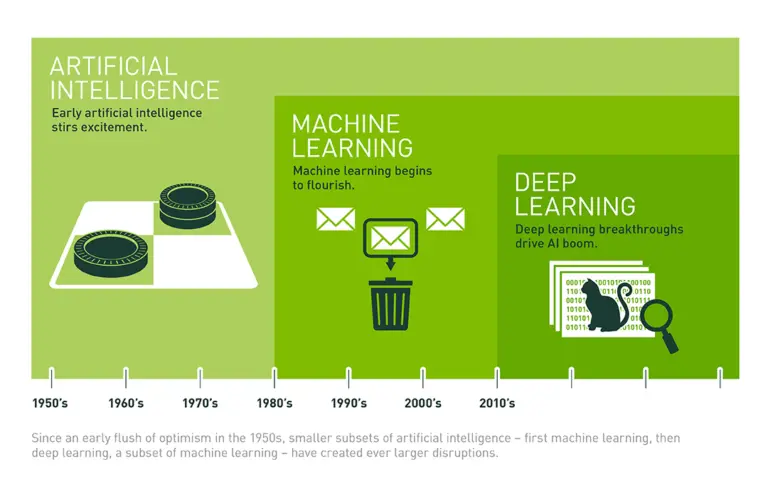
\includegraphics[width=1\linewidth]{Images/aimldl}
	\caption{Mối quan hệ giữa AI, Machine Learning và Deep Learning.
		(Nguồn: \textit{What’s the Difference Between Artificial Intelligence, Machine Learning, and Deep Learning?})}
	\label{fig:aimldl}
\end{figure}
\textbf{Vậy điều gì mang đến sự thành công của deep learning?} Rất nhiều những ý tưởng cơ bản của deep learning được đặt nền móng từ những năm 80-90 của thế kỷ trước, tuy nhiên deep learning chỉ đột phá trong khoảng từ năm 2012. Vì sao?\par
Có thể kể đến một vài nhân tố dẫn đến sự bùng nổ này:
\begin{itemize}
	\item Sự ra đời của các bộ dữ liệu lớn được gán nhãn.
	\item Khả năng tính toán song song tốc độ cao của GPU.
	\item Sự cải tiến của các kiến trúc: GoogLeNet, VGG, ResNet, … và các kỹ thuật transfer learning, fine tuning.
	\item Nhiều thư viện mới hỗ trợ việc huấn luyện deep network với GPU: Theano, Caffe, TensorFlow, PyTorch, Keras,\dots
\end{itemize}

\section{Neural Network - Mạng Neural}
Tổng quan kiến trúc một mạng Neural như sau\par
\begin{figure}[!h]
	\centering
	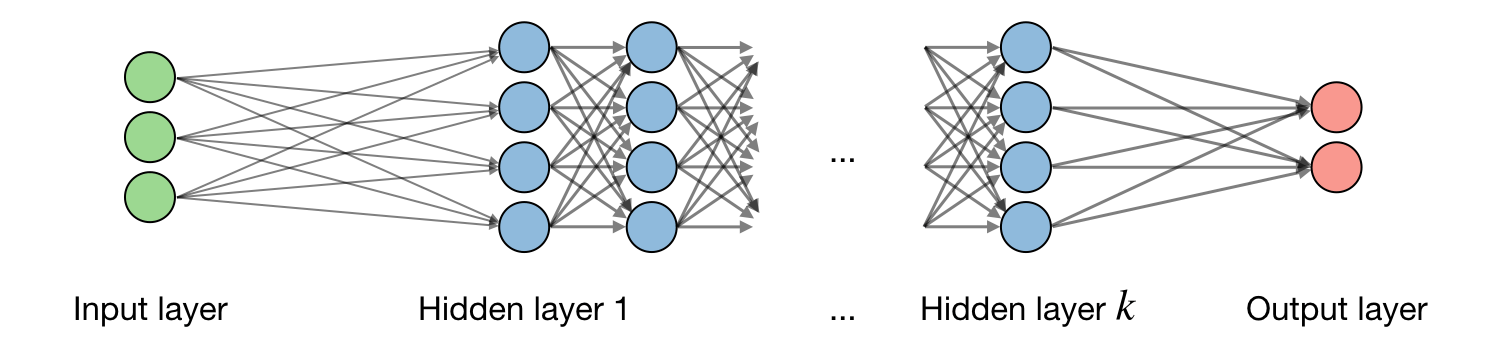
\includegraphics[width=0.8\linewidth]{Images/nn1}
	\caption{Ví dụ một mạng Neural có $k$ tầng ẩn (Nguồn: \textit{CS229})}
	\label{fig:nn1}
\end{figure}
Với $i$ là lớp thứ $i$ của mạng, $j$ là đơn vị ẩn thứ $j$ của lớp, ta có:
$$ z_j^{[i]} = {w_j^{[i]}}^Tx + b_j^{[i]}$$
trong đó: $w$ là weight, $b$ là bias, $z$ là đầu ra. \par
\textbf{Hàm kích hoạt (Activation function):} Bản chất của công thức trên là một tổ hợp tuyến tính giữa các giá trị input $x$ và bộ trọng số $w$, do đó, khi áp dụng chúng với các dữ liệu mà có dạng tuyến tính, tức là dữ liệu mà ta có thể kẻ một đường thẳng để phân cách giữa chúng thì công thức tổ hợp trên đã đủ để giúp cho mô hình máy học có thể hoạt động tốt, chúng ta không cần tới hàm kích hoạt (activation function). Nhưng với các dữ liệu không có dạng tuyến tính, ta không thể kẻ một đường thẳng tuyến tính mà phân tách 2 dữ liệu ra được, và câu hỏi đặt ra là làm thế nào với một công thức tổ hợp tuyến tính như ban đầu mà dùng để phân lớp dữ liệu phi tuyến tính được. \textbf{Hàm kích hoạt} được tạo ra để làm điều này, hàm kích hoạt đóng vai trò như một người trung gian có nhiệm vụ chuyển đổi, nén hoặc chế biến output $z$ từ tuyến tính trở thành phi tuyến tính. \par
\begin{figure}[!h]
	\centering
	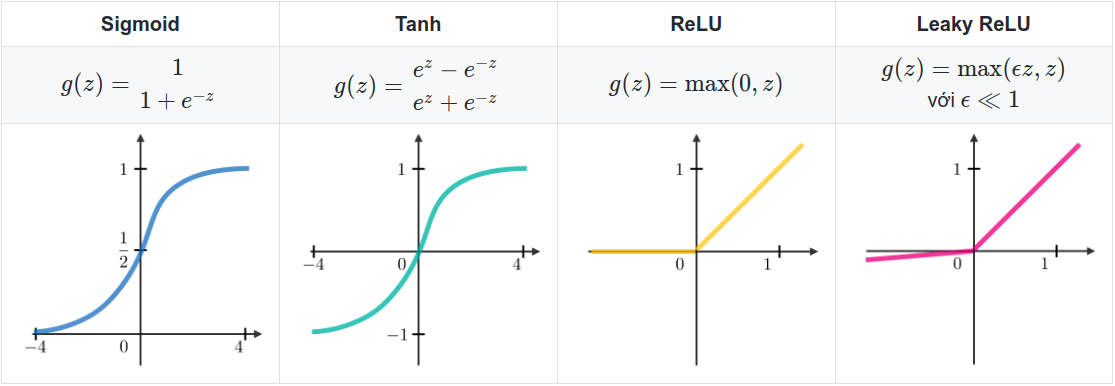
\includegraphics[width=1\linewidth]{Images/nn2}
	\caption{Một số hàm kích hoạt thường dùng (Nguồn: \textit{CS229})}
	\label{fig:nn2}
\end{figure}%\subsubsection{Logistic Regression}
%\textbf{Logistic Regression} là một mô hình thường được áp dụng cho các bài toán phân lớp nhị phân. Trong mô hình này, đầu ra có thể được thể hiện dưới dạng xác suất. Ví dụ, xác suất thi đỗ nếu biết thời gian ôn thi, xác suất ngày mai có mưa dựa trên những thông tin đo được trong ngày hôm nay,\dots Mô hình này có tên là logistic
%regression. Mặc dù trong tên có chứa từ \textit{regression}, logistic regression thường được sử dụng nhiều hơn cho các bài toán phân lớp.\par
%\begin{figure}[!h]
%	\centering
%%	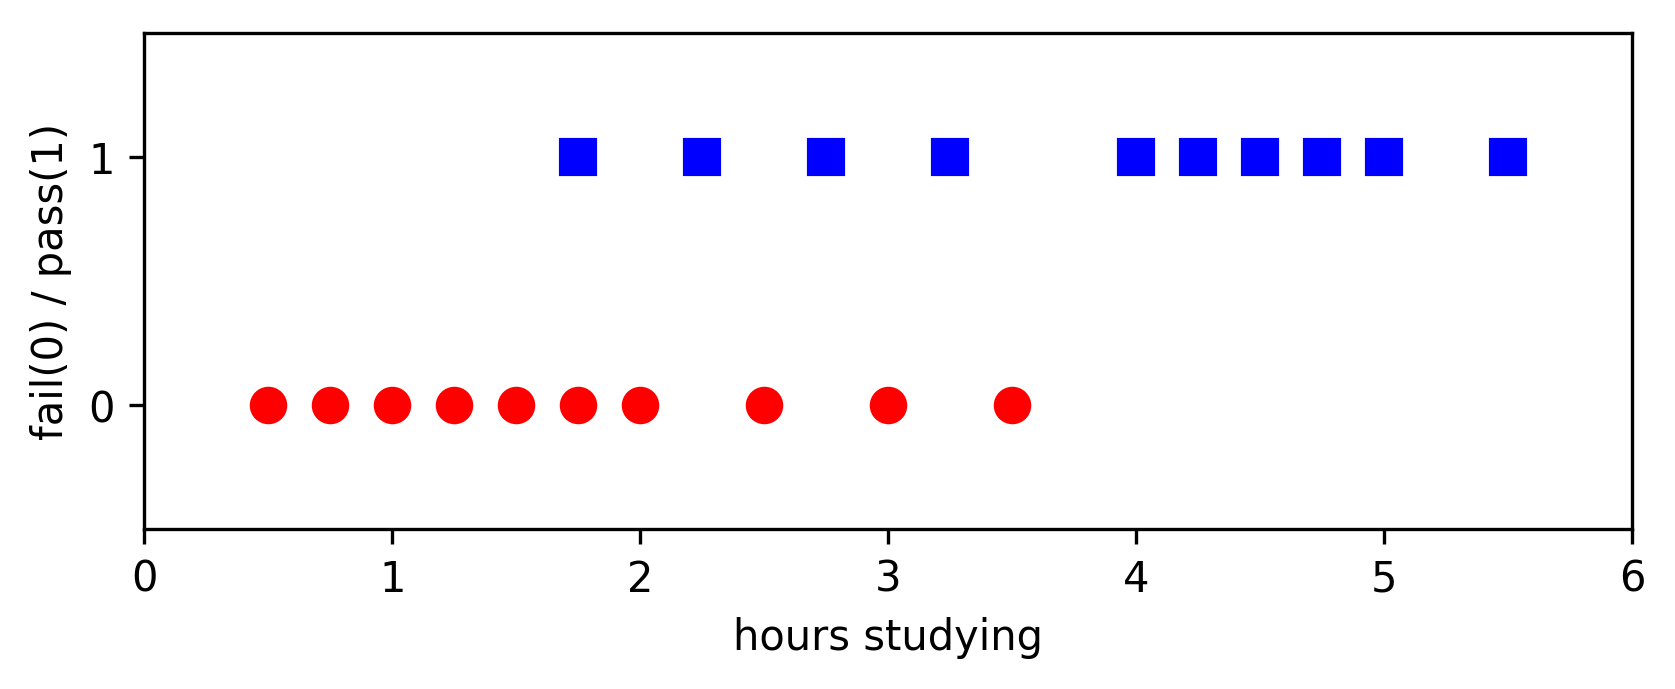
\includegraphics[width=0.7\linewidth]{Images/logit}
%	\caption{Ví dụ về kết quả thi dựa trên số giờ ôn tập (Nguồn: \textit{Machine Learning cơ bản})}
%	\label{fig:logit}
%\end{figure}

\textbf{Hàm mất mát (Loss function):} Hàm mất mát trả về một số thực không âm thể hiện sự chênh lệch giữa hai đại lượng: $y_{pred}$ là giá trị được dự đoán và $y_{true}$ là giá trị thực. Trong trường hợp lý tưởng, $y_{pred} = y_{true}$, hàm mất mát sẽ có giá trị bằng $0$. Hàm loss được sử dụng phổ biến trong các mô hình Deep learning hiện nay là Cross-entropy cùng các biến thể cải tiến của nó (Weighted cross entropy, Focal loss...). Cross-entropy loss $L(z, y)$ được định nghĩa như sau:
$$ L(z, y) = - [ylog{z} + (1-y)log(1-z)]$$ 
\textbf{Optimizer và Learning rate:} Sau khi tính giá trị hàm loss, việc cần làm là tối ưu (cực tiểu hóa) hàm loss và update bộ trọng số $\{w\}$ mới. Learning rate, thường được ký hiệu là $\alpha$ hoặc $\eta$, thể hiện cho tốc độ học hay tốc độ update trọng số. Learning rate có thể là cố định hoặc được thay đổi tuỳ biến trong quá trình học. \par 
\textbf{Lan truyền ngược (Backpropagation):} Lan truyền ngược là phương thức dùng để cập nhật trọng số trong mạng neural bằng cách tính toán đầu ra thực sự và đầu ra mong muốn. Đạo hàm theo trọng số ww được tính bằng cách sử dụng quy tắc chuỗi (chain rule) dưới đây:
$$ \frac{\partial L(z, y)}{\partial w} = \frac{\partial L(z, y)}{\partial a} \times \frac{\partial a}{\partial z} \times \frac{\partial z}{\partial w} $$ 
Như kết quả, trọng số được cập nhật như sau:
$$ w := w - \eta\frac{\partial L(z, y)}{\partial w} $$ 
Tổng kết lại, ta có sơ đồ quá trình học của một mạng neural cơ bản như sau\par
\begin{figure}[!h]
	\centering
	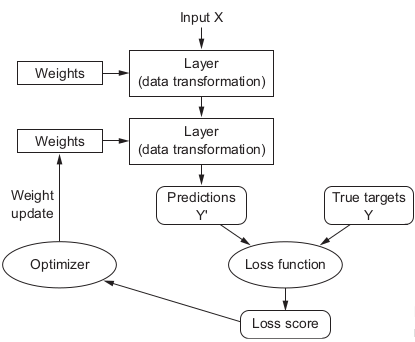
\includegraphics[width=0.8\linewidth]{Images/nn3}
	\caption{Mối quan hệ giữa network, layers, loss function và optimizer (Nguồn: Deep Learing with Python - Francois Chollet)}
	\label{fig:nn3}
\end{figure}

\section{Mạng Neural tích chập (Convolutional Neural Network - CNN)}
Mạng Neural tích chập là một trong những mô hình Deep learning phổ biến nhất và có ảnh hưởng nhiều nhất trong lĩnh vực Computer Vision. CNNs được dùng trong trong nhiều bài toán như nhân dạng ảnh, phân tích video, ảnh MRI, hoặc có thể cho cả các bài của lĩnh vự xử lý ngôn ngữ tự nhiên, và hầu hết đều giải quyết tốt các bài toán này.\par
Mạng neural tích chập, còn được biết đến với tên CNNs, là một dạng mạng neural được cấu thành bởi các layer sau:\par
\begin{figure}[!h]
	\centering
	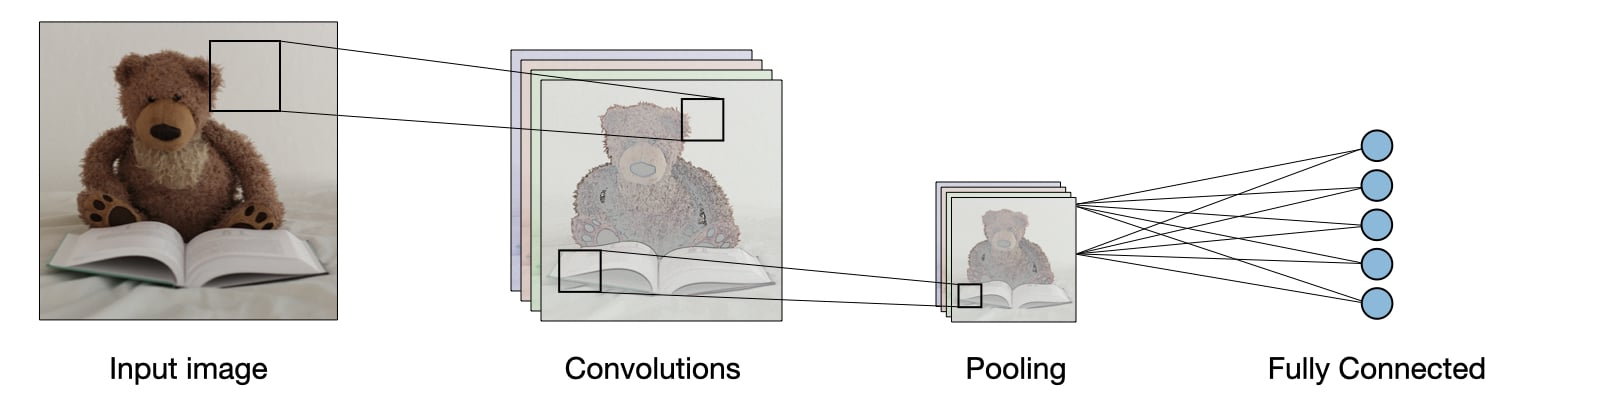
\includegraphics[width=1\linewidth]{Images/cnn1}
	\caption{Ví dụ về một CNN (Nguồn: \textit{CS230})}
	\label{fig:nn3}
\end{figure}
\textbf{Lớp tích chập (Convolution layer):} Tầng tích chập (CONV) sử dụng các bộ lọc (filters) để thực hiện phép tích chập khi đưa chúng đi qua input $I$ theo các chiều của nó. Các \textit{hyperparameters} của filter bao gồm  kích thước $F$, độ trượt (stride) $S$. Kết quả đầu ra của lớp này được gọi là feature map.\par
\begin{figure}[!h]
	\centering
	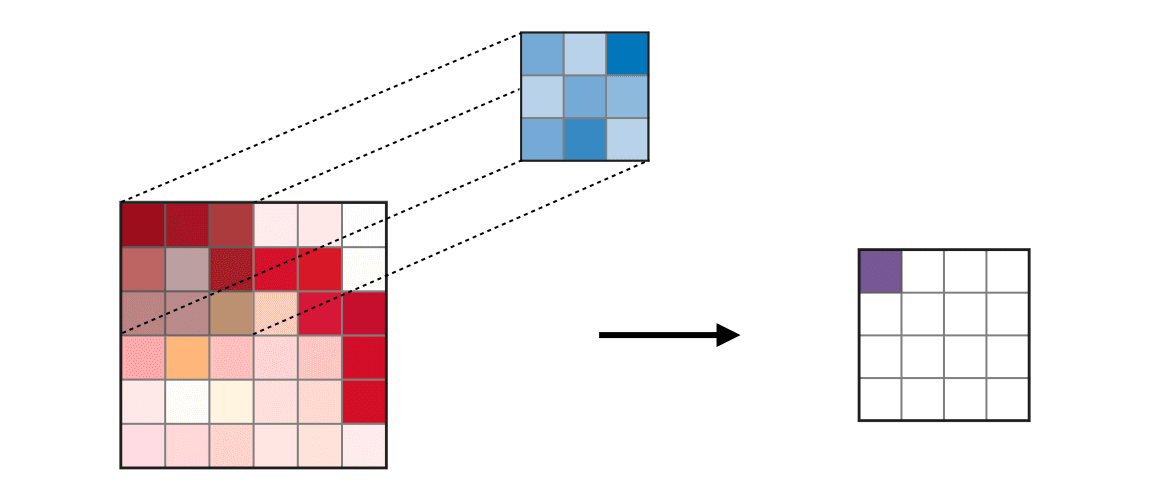
\includegraphics[width=1\linewidth]{Images/cnn2}
	\caption{Mô tả hoạt động của CONV (Nguồn: \textit{CS230})}
	\label{fig:cnn2}
\end{figure}
\textbf{Stride} là số lượng pixel dịch chuyển trên ma trận đầu vào hay Stride dùng để dịch chuyển filter theo mỗi bước xác định.\par
\begin{center}
\begin{minipage}{4cm}
	\centering
	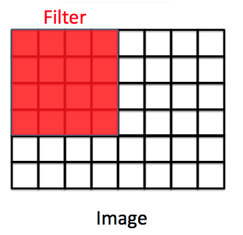
\includegraphics[scale=0.5]{Images/stride1}
\end{minipage}
\begin{minipage}{4cm}
	\centering
	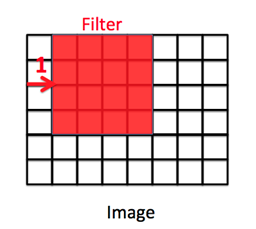
\includegraphics[scale=0.425]{Images/stride2}
\end{minipage}
\begin{minipage}{4cm}
	\centering
	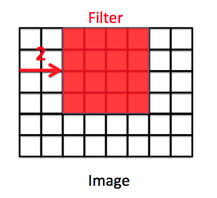
\includegraphics[scale=0.5]{Images/stride3}
\end{minipage}

Ví dụ về stride = 1 và stride bằng 2
\end{center}
\textbf{Padding:} Khi áp dụng phép CONV thì ma trận đầu vào sẽ có nhỏ dần đi, do đó số layer của mô hình CNN sẽ bị giới hạn, và không thể xậy đựng mô hình mong muốn. Để giải quyết tình trạng này, ta cần "bọc" bên ngoài ma trận đầu vào để đảm bảo kích thước đầu ra sau mỗi tầng convolution là không đổi. Do đó có thể xậy dựng được mô hình với số tầng convolution lớn tùy ý. Một cách đơn giản và phổ biến nhất để padding là sử dụng hàng số 0, ngoài ra có một số phương pháp khác như reflection padding hay là symmetric padding. \par
\textbf{Lớp Pooling:} Pooling layer thường được dùng giữa các convolutional layer, để giảm kích thước dữ liệu nhưng vẫn giữ được các thuộc tính quan trọng. Kích thước dữ liệu giảm giúp giảm việc tính toán trong model.\par
\textbf{Spatial pooling} được gọi là lấy mẫu con làm giảm chiều của mỗi map nhưng vẫn giữ được thông tin quan trọng. Spatial pooling có thể có nhiều loại khác nhau như Max Pooling và Average Pooling. \par
\begin{figure}[!h]
	\centering
	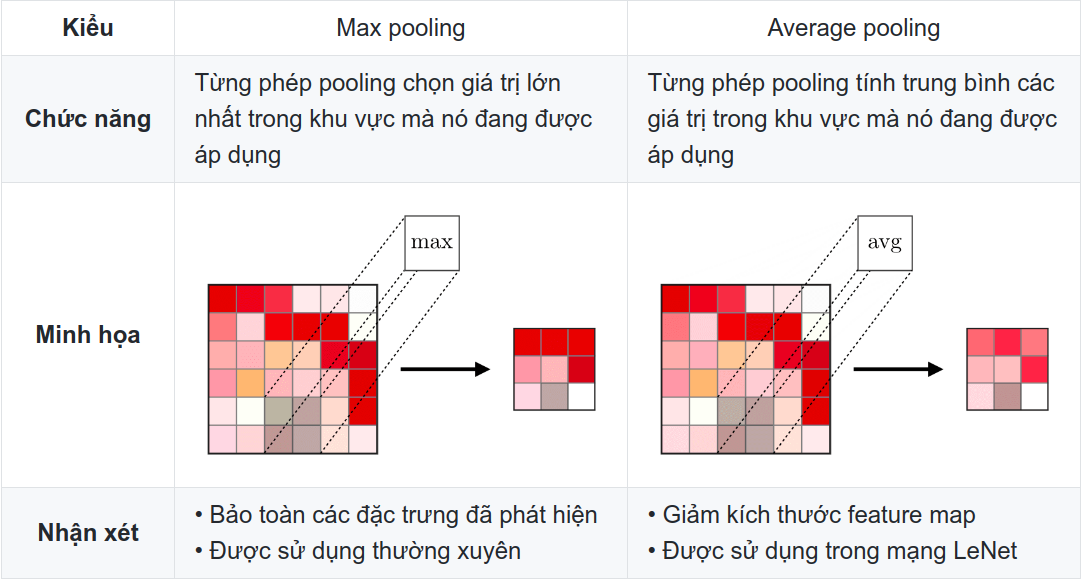
\includegraphics[width=0.9\linewidth]{Images/pooling}
	\caption{Hai kiểu pooling phổ biến (Nguồn: \textit{CS230})}
	\label{fig:pooling}
\end{figure}
\textbf{Fully Connected (FC):} Lớp Fully Connected nhận đầu vào là các dữ liệu đã được làm phẳng, mà mỗi đầu vào đó được kết nối đến tất cả neural. Trong mô hình mạng CNNs, các lớp FC thường được tìm thấy ở cuối mạng và được dùng để tối ưu hóa mục tiêu của mạng ví dụ như độ chính xác của lớp. \par
\begin{figure}[!h]
	\centering
	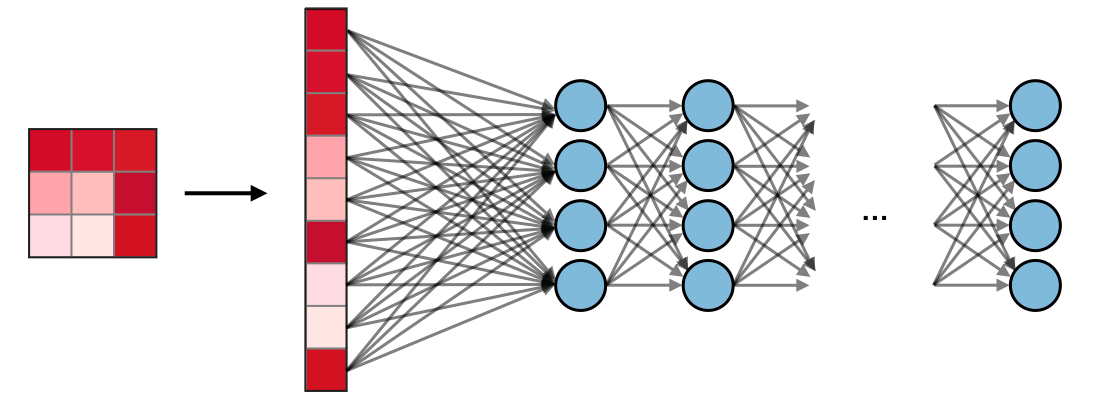
\includegraphics[width=0.9\linewidth]{Images/fc}
	\caption{Fully Connected layer (Nguồn: \textit{CS230})}
	\label{fig:fc}
\end{figure}
\textbf{Các hàm kích hoạt thường gặp:} 
\begin{itemize}
	\item \textbf{Rectified Linear Unit (ReLU)}: ReLU là một hàm kích hoạt $g$ được sử dụng trên tất cả các thành phần. Mục đích của nó là tăng tính phi tuyến tính cho mạng. Những biến thể khác của ReLU được tổng hợp ở bảng dưới\par
	\begin{figure}[h!]
		\centering
		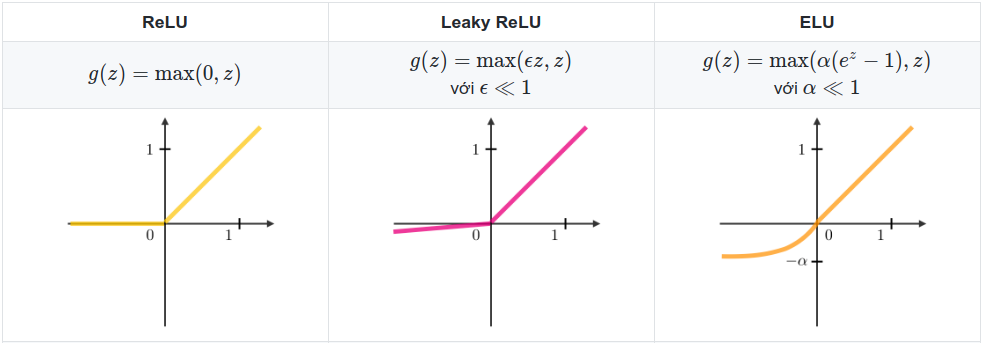
\includegraphics[width=1\linewidth]{Images/relu1}
		\caption{ReLU và biến thể (Nguồn: \textit{CS230})}
		\label{fig:relu1}
	\end{figure}
	\item \textbf{Softmax:} Bước softmax có thể được coi là một hàm logistic tổng quát lấy đầu vào là một vector chứa các giá trị $x \in \mathbb{R}^n$ và cho ra là một vector gồm các xác suất $p \in \mathbb{R}^n$ thông qua một hàm softmax ở layer cuối.
	$$ p = (p_1,\dots,p_n)^T \text{ trong đó } p = \frac{e^{x_i}}{\displaystyle\sum_{j=1}^ne^{x_j}} $$
\end{itemize}

\section{Bài toán nhận diện vật thể (Object Detection)}
Các hình ảnh trong cuộc sống bình thường thì không chỉ chứa 1 đối tượng mà thường bao gồm rất nhiều các đối tượng. Ta quan tâm đến vị trí của từng đối tượng trong ảnh. Bài toán như vậy được gọi là: object detection.\par
\begin{figure}[!h]
	\centering
	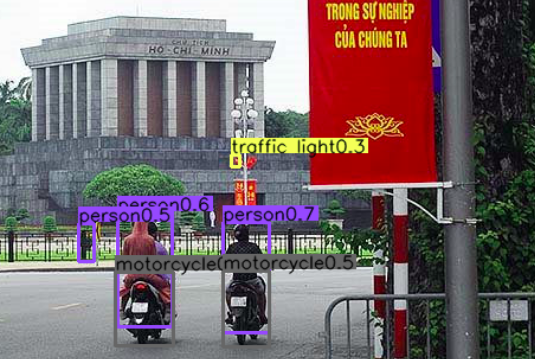
\includegraphics[width=0.7\linewidth]{Images/det}
	\caption{Ví dụ về đầu ra của bài toán nhận diện vật thể}
	\label{fig:det}
\end{figure}
Bài toán object detection có input là ảnh màu và output là vị trí của các đối tượng trong ảnh. Ta thấy nó bao gồm 2 bài toán nhỏ:
\begin{itemize}
	\item Xác định các bounding box (hình chữ nhật) quanh đối tượng.
	\item Với mỗi bouding box thì cần phân loại xem đấy là đối tượng gì (người, mèo, ô tô,…) với bao nhiêu phần trăm chắc chắn.
\end{itemize}
Object Detection là 1 bài toán đã đạt được rất nhiều các thành tựu trong những năm gần đây, cả phần ứng dụng và mô hình thuật toán. Điển hình là các phương pháp Object Detection sử dụng Deep Learning đã đạt được các bước cải thiện vượt trội so với các phương pháp xử lý ảnh thông thường khác.\par
Có hai loại bài toán Object detection: two-stage object detection và one-stage object detection.\par
\textbf{Two-stage object detection:} Điển hình họ các thuật toán R-CNN. Việc gọi là two-stage là do cách model xử lý để lấy ra được các vùng có khả năng chứa vật thể từ bức ảnh. Ví dụ, với Faster-RCNN thì trong stage-1, ảnh sẽ được đưa ra 1 sub-network gọi là RPN (Region Proposal Network) với nhiệm vụ extract các vùng trên ảnh có khả năng chứa đối tượng dựa vào các anchor. Sau khi đã thu được các vùng đặc trưng từ RPN, model Faster-RCNN sẽ thực hiện tiếp việc phân loại đối tượng và xác định vị trí nhờ vào việc chia làm 2 nhánh tại phần cuối của mô hình (Object classification \& Bounding box regression).\par
\textbf{One-stage Object Detection:} Các thuật toán điển hình như: SSD, YOLO, RetinaNet. Gọi là one-stage vì trong việc thiết kế model hoàn toàn không có phần trích chọn các vùng đặc trưng (các vùng có khả năng chứa đối tượng) như RPN của Faster-RCNN. Các mô hình one-stage object detection coi phần việc phát hiện đối tượng (object localization) như một bài toán regression (với 4 tọa độ offset, ví dụ x, y, w, h) và cũng dựa trên các box được định nghĩa sẵn gọi là anchor để làm việc đó. Các mô hình dạng này thường nhanh hơn tuy nhiên "độ chính xác" của model thường kém hơn so với two-stage object detection. Tuy nhiên, một số mô hình one-stage vẫn tỏ ra vượt trội hơn một chút so với two-stage như Retina-Net với việc việc thiết kế mạng theo FPN (Feature Pyramid Network) và Focal Loss.\par
\subsection{Mô hình Faster R-CNN}
\subsubsection{Regions with CNN features (R-CNN)}
R-CNN được giới thiệu lần đầu vào 2014 bởi Ross Girshick và các cộng sự ở UC Berkeley một trong những trung tâm nghiên cứu AI hàng đầu thế giới trong bài báo \textit{Rich feature hierarchies for accurate object detection and semantic segmentation}. RCNN có thể là xem một trong những ứng dụng nền móng đầu tiên của CNN đối với bài toán định vị, phát hiện và phân đoạn đối tượng. \par
Kiến trúc của R-CNN gồm 3 thành phần đó là:
\begin{itemize}
	\item Vùng đề xuất hình ảnh (Region proposal): Có tác dụng tạo và trích xuất các vùng đề xuất chứa vật thể được bao bởi các bounding box.
	\item Trích lọc đặc trưng (Feature Extractor): Trích xuất các đặc trưng giúp nhận diện hình ảnh từ các region proposal thông qua các CNN.
	\item Phân loại (classifier): Dựa vào input là các features ở phần trước để phân loại hình ảnh chứa trong region proposal về đúng nhãn.
\end{itemize}\par
\begin{figure}[h!]
	\centering
	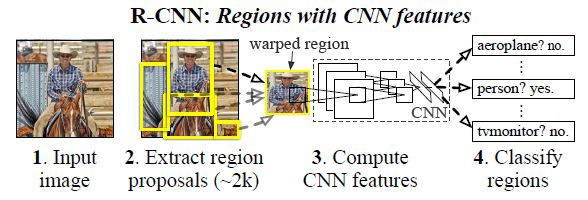
\includegraphics[width=1\linewidth]{Images/rcnn}
	\caption{Sơ đồ xử lý trong mô hình mạng R-CNN (Nguồn: \textit{Medium})}
	\label{fig:rcnn}
\end{figure}

\begin{figure}[!h]
	\centering
	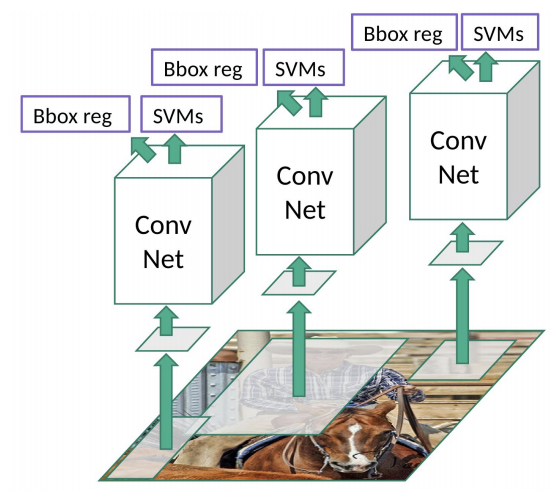
\includegraphics[width=0.45\linewidth]{Images/rcnn1}
	\caption{R-CNN (Nguồn: \textit{Medium})}
	\label{fig:rcnn1}
\end{figure}

Để vượt qua vấn đề chọn một số lượng lớn các region, Ross Girshick đề xuất một phương pháp gọi là selective search để chỉ trích xuất 2000 regions từ hình ảnh và gọi chúng là vùng đề xuất (region proposals), tức vùng có khả năng chứa đối tượng. Do đó, thay vì cố gắng phân loại một số lượng lớn các region, ta chỉ cần làm việc với 2000 regions. 2000 propsal regions này được uốn cong thành một hình vuông và được đưa vào một mạng CNN tạo ra một vector đặc trưng 4096 chiều làm đầu ra. CNN hoạt động như một công cụ trích xuất đặc trưng và dense layer đầu ra bao gồm các đặc trưng được trích xuất từ các ảnh và các đặc trưng được đưa vào một SVM để phân loại sự hiện diện của đối tượng trong proposal region được lấy ra đó. Ngoài việc dự đoán sự hiện diện của một đối tượng trong các proposal region, thuật toán cũng dự đoán bốn giá trị là độ lệch (offset values) để tăng độ chính xác của bounding box, Ví dụ với một region proposal cho trước, thuật toán sẽ dự đoán sự hiện diện của người nhưng khuôn mặt người đó trong region proposal đó có thể bị cắt đi một nửa. Do đó, các giá trị bù giúp điều chỉnh bounding box của region proposal.\par
\textbf{Nhược điểm của R-CNN:}
\begin{itemize}
	\item Vẫn tốn lượng lớn thời gian để luyện mạng vì phải phân loại 2000 region proposals mỗi ảnh.
	\item Không thể chạy với thời gian thực do nó tốn thời gian 47 giây cho mỗi ảnh
	\item Thuật toán selective search là một thuật toán cố định. Do đó, không có việc học nào đang diễn ra ở giai đoạn đó, Điều này có thể dẫn đến việc tạo ra các region proposal tồi.
\end{itemize}
\subsubsection{Fast R-CNN}
Dựa trên thành công của R-CNN, Ross Girshick (lúc này đã chuyển sang Microsoft Research) đề xuất một mở rộng để giải quyết vấn đề của R-CNN trong một bài báo vào năm 2015 với tiêu đề rất ngắn gọn Fast R-CNN.\par
Tương tự như R-CNN thì Fast R-CNN vẫn dùng selective search để lấy ra các region proposal. Tuy nhiên là nó không tách 2000 region proposal ra khỏi ảnh và thực hiện bài toán image classification cho mỗi ảnh. Fast R-CNN cho cả bức ảnh vào ConvNet (một vài convolutional layer + max pooling layer) để tạo ra convolutional feature map. Sau đó các vùng region proposal được lấy ra tương ứng từ convolutional feature map. Tiếp đó được Flatten và thêm 2 Fully connected layer (FCs) để dự đoán lớp của region proposal và offset values của bounding box.\par
\begin{figure}[!h]
	\centering
	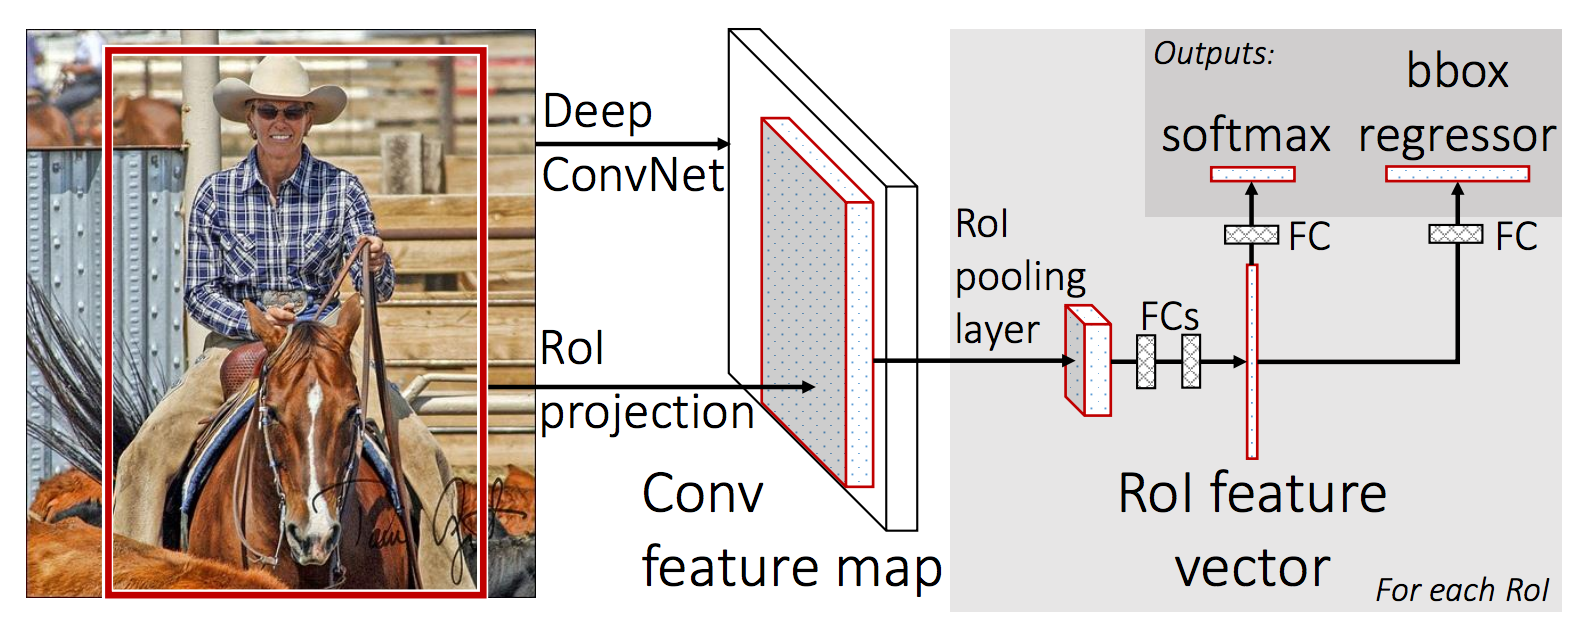
\includegraphics[width=0.7\linewidth]{Images/fastrcnn}
	\caption{Fast R-CNN (Nguồn: \textit{Medium})}
	\label{fig:fastrcnn}
\end{figure}
Tuy nhiên là kích thước của các region proposal khác nhau nên khi Flatten sẽ ra các vector có kích thước khác nhau nên không thể áp dụng neural network được. Với R-CNN, nó đã resize các region proposal về cùng kích thước trước khi dùng transfer learning. Tuy nhiên ở feature map ta không thể resize được, nên ta phải có cách gì đấy để chuyển các region proposal trong feature map về cùng kích thước nên \textbf{Region of Interest (RoI) pooling} ra đời.\par
\textbf{Region of Interest (RoI) pooling:} RoI pooling là một dạng của pooling layer. Điểm khác so với max pooling hay average pooling là bất kể kích thước của tensor input, RoI pooling luôn cho ra output có kích thước cố định được định nghĩa trước.\par
\begin{figure}[!h]
	\centering
	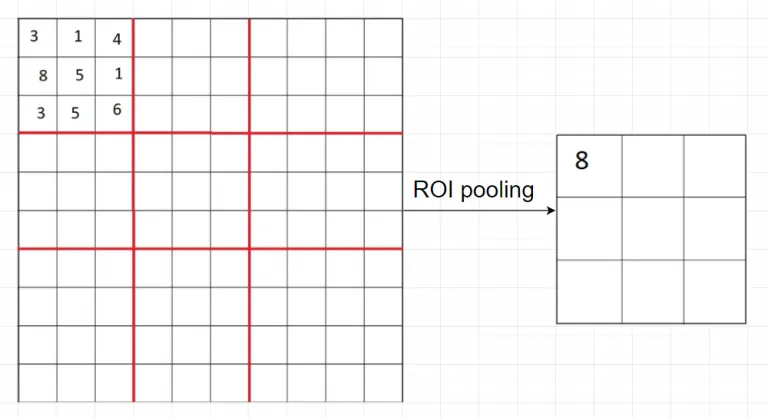
\includegraphics[width=0.7\linewidth]{Images/roi}
	\caption{RoI pooling (Nguồn: \textit{nttuan8.com})}
	\label{fig:roi}
\end{figure}
Fast R-CNN khác với R-CNN là nó thực hiện feature map với cả ảnh sau đó với lấy các region proposal ra từ feature map, còn R-CNN thực hiện tách các region proposal ra rồi mới thực hiện CNN trên từng region proposal. Do đó Fast R-CNN nhanh hơn đáng kể nhờ tối ưu việc tính toán bằng Vectorization. \par
\begin{figure}[!h]
	\centering
	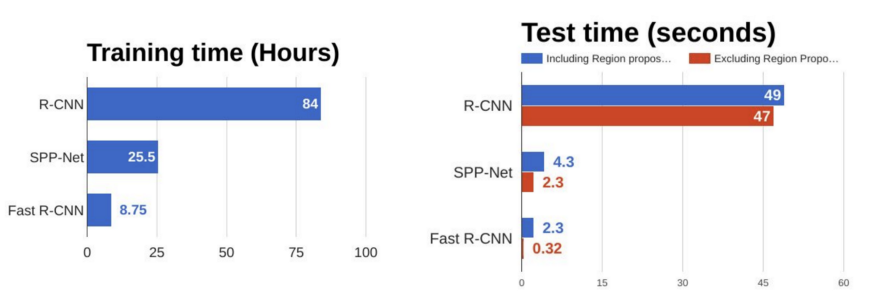
\includegraphics[width=1\linewidth]{Images/time}
	\caption{So sánh một số thuật toán object detection (Nguồn: \textit{towardsdatascience.com})}
	\label{fig:time}
\end{figure}
Tuy nhiên nhìn hình trên ở phần test time với mục Fast R-CNN thì thời gian tính region proposal rất lâu và làm chậm thuật toán. Do đó cần thay thế thuật toán selective search và việc dùng Deep learning để tao ra region proposal được thực hiện với mô hình Faster R-CNN.\par
\subsubsection{Faster R-CNN}
Faster R-CNN không dùng thuật toán selective search để lấy ra các region proposal, mà nó thêm một mạng CNN mới gọi là Region Proposal Network (RPN) để tìm các region proposal.\par
\begin{figure}[!h]
	\centering
	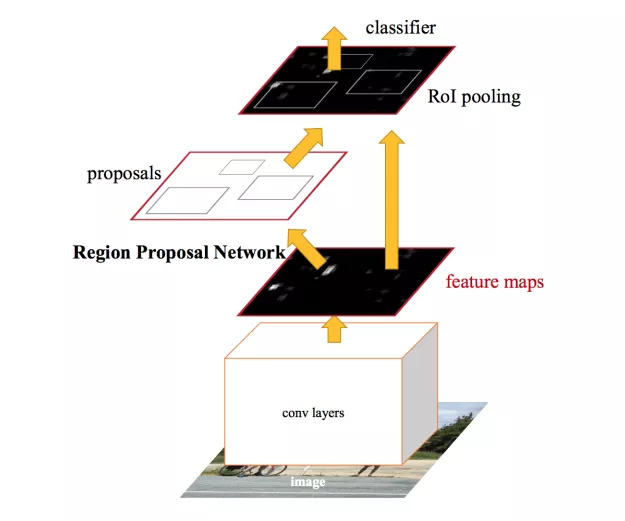
\includegraphics[width=0.7\linewidth]{Images/fasterrcnn}
	\caption{Mô hình Faster R-CNN (Nguồn: \textit{arXiv:1506.01497})}
	\label{fig:fasterrcnn}
\end{figure}
%\begin{figure}[!h]
%	\centering
%	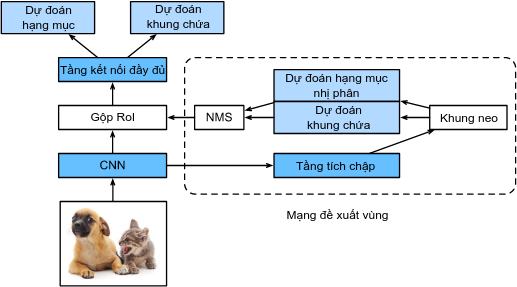
\includegraphics[width=0.7\linewidth]{Images/fasterrcnn1}
%	\caption{Mô hình Faster R-CNN. (Nguồn: \textit{d2l.aivivn.com})}
%	\label{fig:fasterrcnn1}
%\end{figure}

Một Region Proposal Network nhận đầu vào là ảnh với kích thước bất kì và cho đầu ra là region proposal (tập vị trí của các hình chữ nhật có thể chứa vật thể), cùng với xác suất chứa vật thể của hình chữ nhật tương ứng. \par
\textbf{Region Proposal Network (RPN):} Quy trình tính toán của RPN được mô tả chi tiết dưới đây: 
\begin{enumerate}
	\item Dùng một lớp tích chập $3\times 3$ với padding bằng 1 để biến đổi đầu ra của CNN và đặt số kênh đầu ra bằng $c$. Bằng cách này phần tử trong feature map mà CNN trích xuất ra từ bức ảnh là một đặc trưng mới có độ dài bằng $c$.
	\item Lấy mỗi phần tử trong feature map làm tâm để tạo ra nhiều anchor box có kích thước và tỷ lệ khác nhau, sau đó gán nhãn cho chúng.  
	\item Lấy những đặc trưng của các phần tử có độ dài $c$ ở tâm của anchor box để phân loại nhị phân (là vật thể hay là nền) và dự đoán bounding box tương ứng cho các anchor box.
	\item Sau đó, sử dụng non-maximum suppression để loại bỏ các bounding box có kết quả giống nhau của hạng mục “vật thể”. Cuối cùng, ta xuất ra các bounding box dự đoán là các proposal region rồi đưa vào lớp RoI pooling.
\end{enumerate}
Vì là một phần của mô hình Faster R-CNN, nên RPN được huấn luyện cùng với phần còn lại trong mô hình. Ngoài ra, trong đối tượng Faster R-CNN còn chứa các hàm dự đoán hạng mục và bounding box trong bài toán phát hiện vật thể, cũng như các hàm dự đoán hạng mục nhị phân và bounding box cho các anchor box trong RPN. Sau cùng, RPN có thể học được cách sinh ra những proposal region có chất lượng cao, giảm đi số lượng proposal region trong khi vẫn giữ được độ chính xác khi phát hiện vật thể.\par
\begin{figure}[!h]
	\centering
	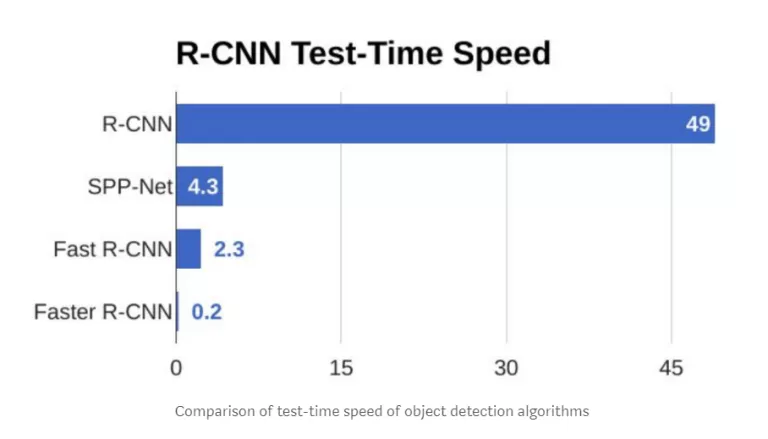
\includegraphics[width=0.7\linewidth]{Images/fasterrcnn2}
	\caption{Faster R-CNN nhanh hơn hẳn các dòng R-CNN trước đó, vì vậy có thể dùng cho real-time objec detection (Nguồn: \textit{nttuan8.com})}
	\label{fig:fasterrcnn2}
\end{figure}
\subsection{Một số phương pháp đánh giá mô hình nhận diện vật thể}
\subsubsection{Intersection over Union (IoU)}
Intersection over Union là chỉ số đánh giá được sử dụng để đo độ chính xác của Object detector trên tập dữ liệu cụ thể. IoU đơn giản chỉ là một chỉ số đánh giá. Mọi thuật toán có khả năng predict ra các bounding box làm output đều có thể được đánh giá thông qua IoU. \par
\begin{figure}[!h]
	\centering
	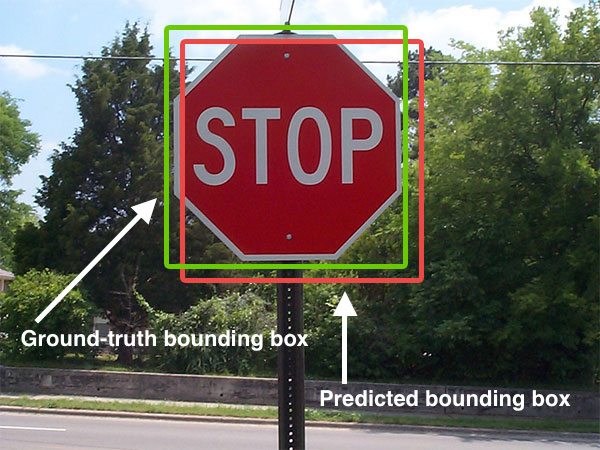
\includegraphics[width=0.5\linewidth]{Images/iou1}
	\caption{Một ví dụ về phát hiện biển báo Stop từ hình ảnh. (Nguồn: \textit{pyimagesearch.com})}
	\label{fig:iou1}
\end{figure}
Để áp dụng được IoU để đánh giá một mô hình nhận diện vật thể bất kì ta cần:
\begin{itemize}
	\item Những ground-truth bounding box (bounding box đúng của đối tượng, ví dụ như bounding box của đối tượng được khoanh vùng và gán nhãn bằng tay sử dụng trong tập test.)
	\item Những bounding box dự đoán được model sinh ra.
\end{itemize}
\begin{figure}[!h]
	\centering
	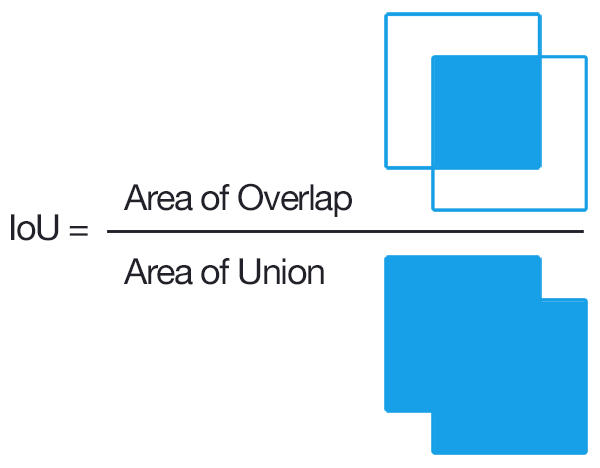
\includegraphics[width=0.5\linewidth]{Images/iou3}
	\caption{Tính toán Intersection over Union. (Nguồn: \textit{pyimagesearch.com})}
	\label{fig:iou3}
\end{figure}
\begin{figure}[!h]
	\centering
	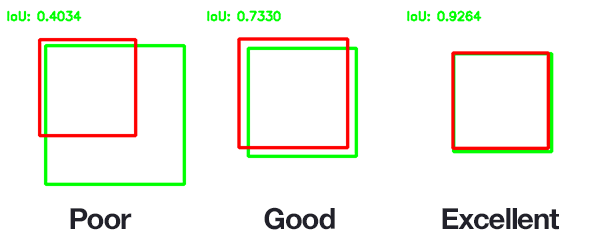
\includegraphics[width=0.7\linewidth]{Images/iou4}
	\caption{Một ví dụ về tính toán IoU cho những bounding box khác nhau. (Nguồn: \textit{pyimagesearch.com})}
	\label{fig:iou4}
\end{figure}

\subsubsection{Average Precision}
AP (Average Precision) là một metric phổ biến trong việc đánh giá độ chính xác của các mô hình nhận diện vật thể như aster R-CNN, SSD,\dots\par	
\textbf{Precison $-$ Recall}\\
Với bài toán phân loại mà tập dữ liệu của các lớp là chênh lệch nhau rất nhiều, có một phép đó hiệu quả thường được sử dụng là Precision-Recall.\par
Trước hết xét bài toán phân loại nhị phân. Ta cũng coi một trong hai lớp là positive, lớp còn lại là negative.\par
\begin{figure}[!h]
	\centering
	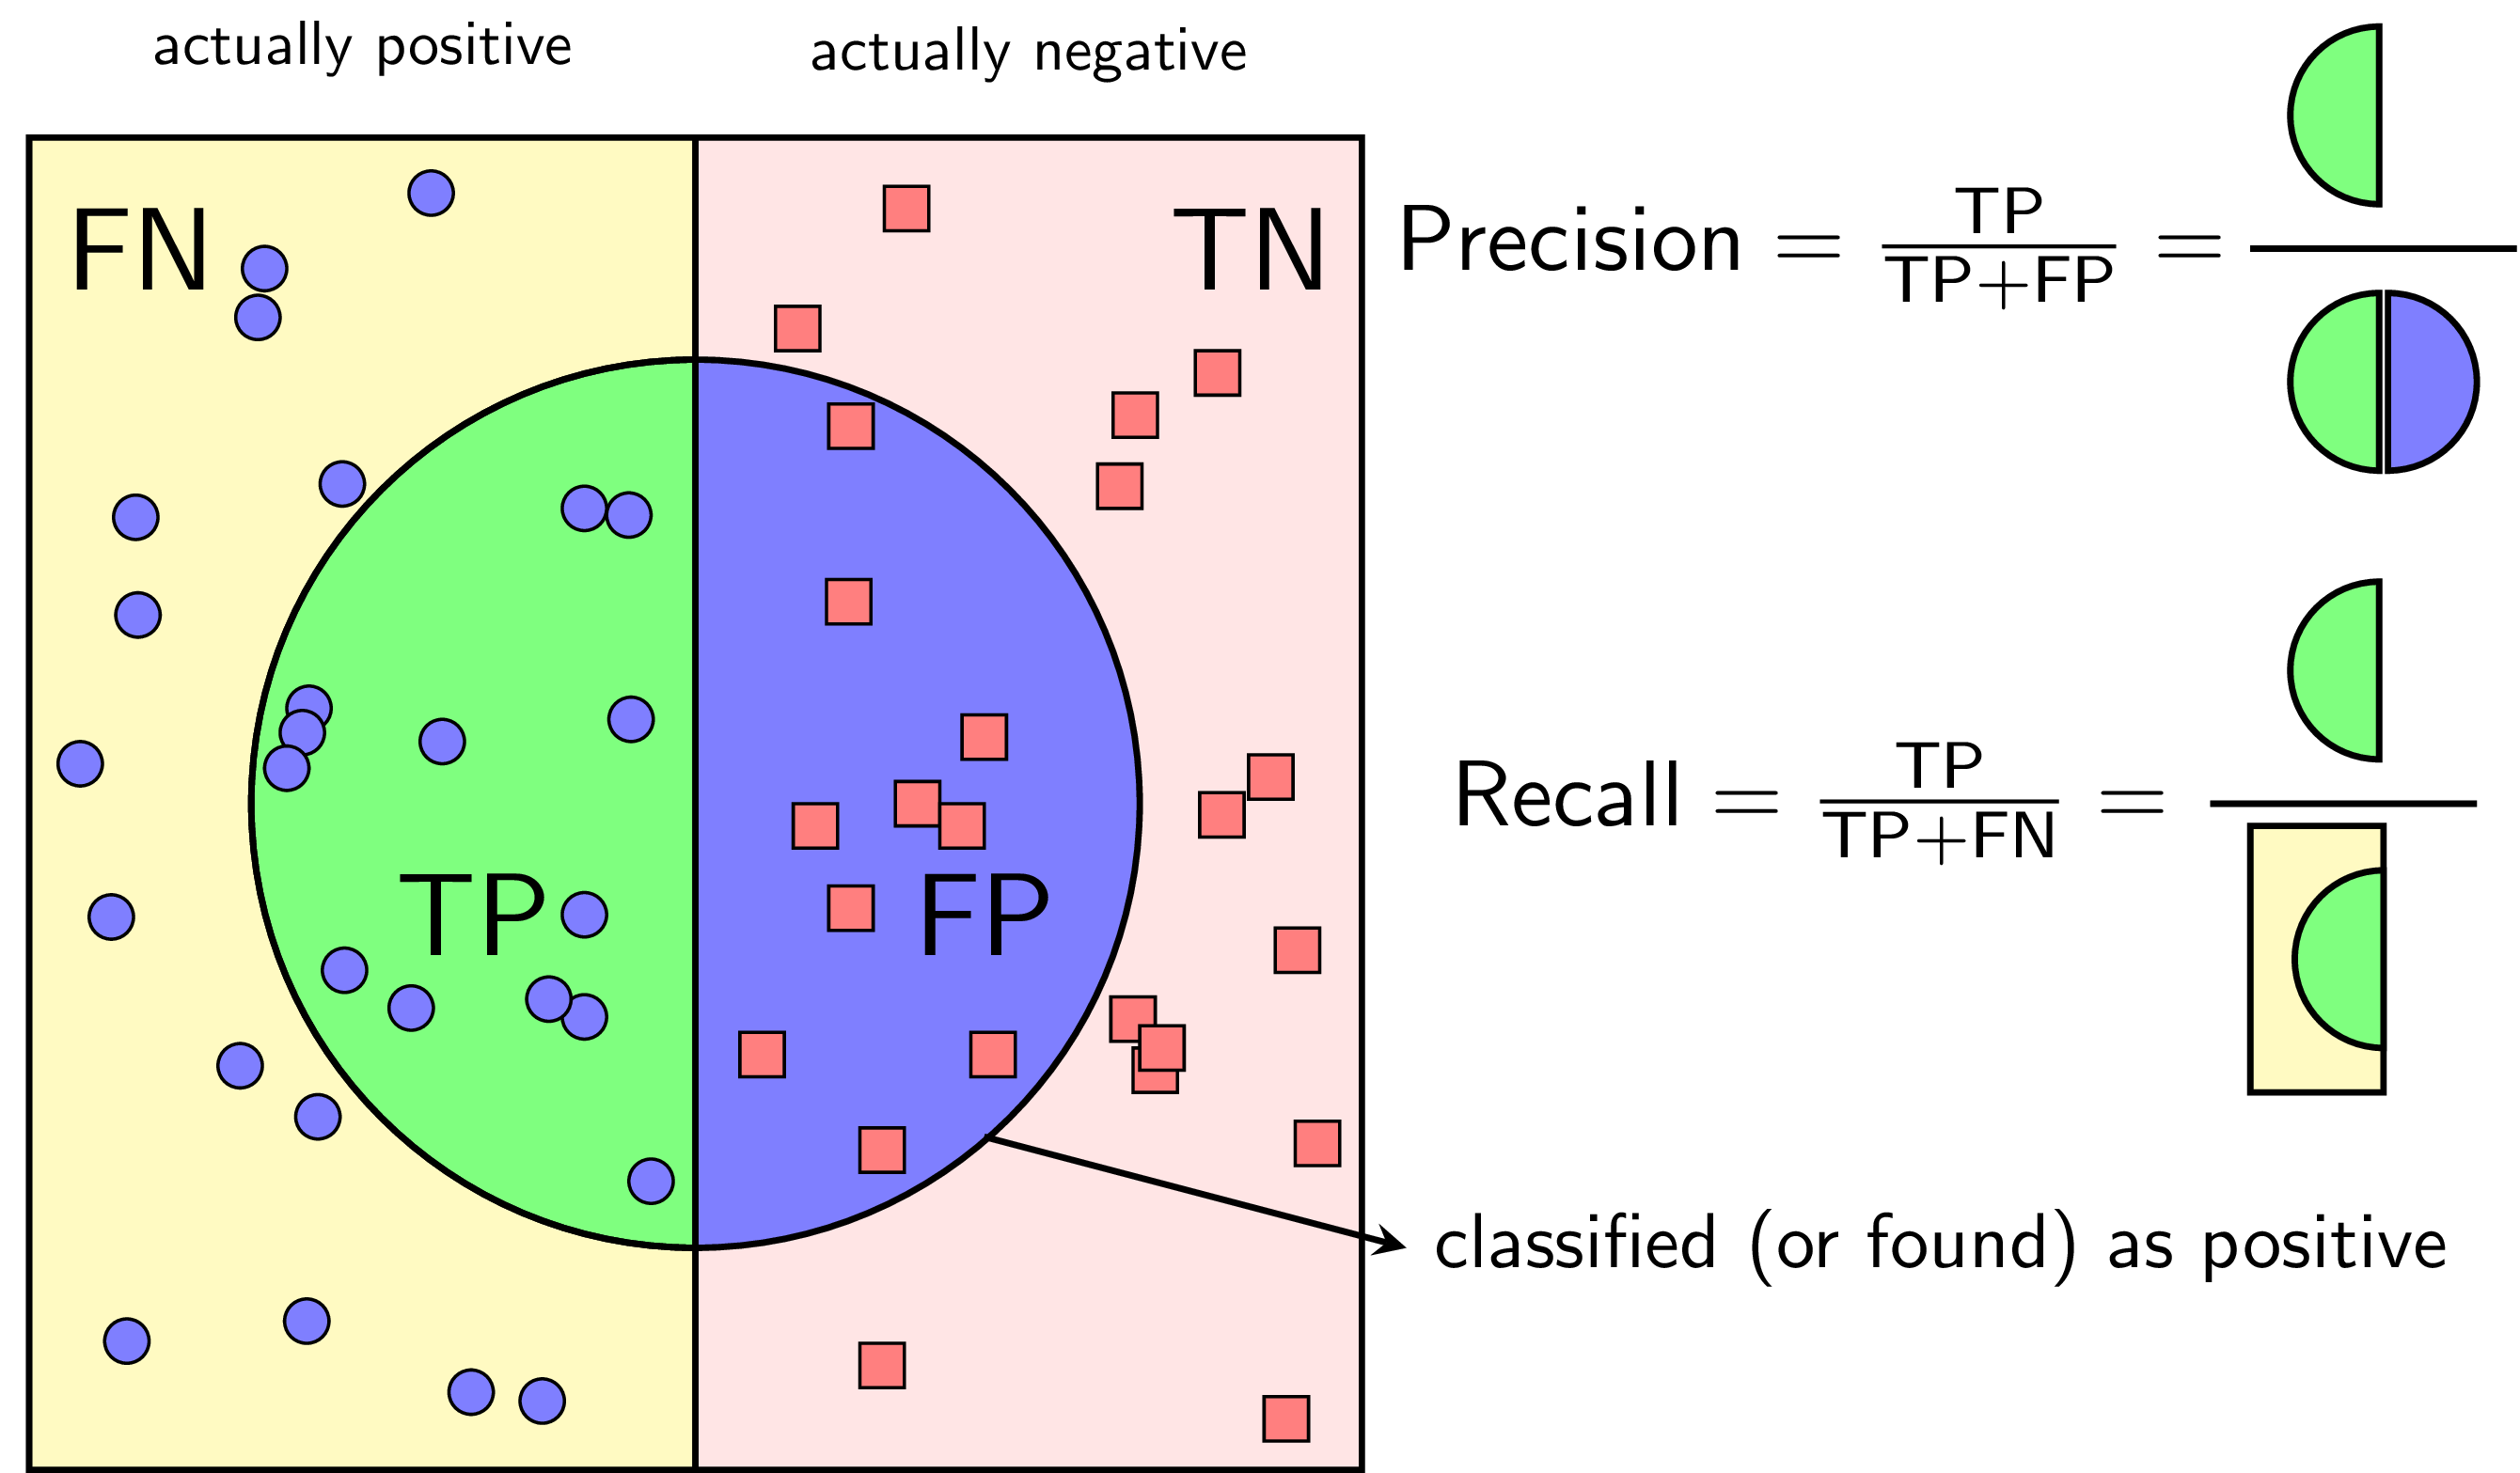
\includegraphics[width=0.7\linewidth]{Images/PR}
	\caption{Cách tính Precision và Recall. (Nguồn: \textit{Machine Learning cơ bản})}
	\label{fig:iou2}
\end{figure}
\textbf{Precision} cao đồng nghĩa với việc độ chính xác của các điểm tìm được là cao. \textbf{Recall} cao đồng nghĩa với việc True Positive Rate cao, tức tỉ lệ bỏ sót các điểm thực sự positive là thấp.\par
\textbf{Precision-Recall curve và Average precision}\\
Ta có thể đánh giá mô hình dựa trên việc thay đổi một ngưỡng và quan sát giá trị của Precision và Recall.\par
\textbf{Average Precision:} Ta xét một ví dụ, với bộ dữ liệu có 5 quả táo, mô hình lần lượt đưa ra 10 dự đoán, ta chọn ngưỡng cho dự đoán đúng là IoU > 0.5, dự đoán được xếp giảm dần theo sự 'tự tin' của dự đoán. Số liệu được thể hiện trong bảng sau: \par
	\begin{center}
		\begin{tabular}{||c c c c ||} 
			\hline
			Rank & Correct? & Precision & Recall \\ [0.5ex] 
			\hline\hline
			1 & True & 1.0 & 0.2   \\ 
			\hline
			2 & True & 1.0 & 0.4   \\
			\hline
			3 & False & 0.67 & 0.4 \\
			\hline
			4 & False & 0.5 & 0.4  \\
			\hline
			5 & False & 0.4 & 0.4  \\ 
			\hline
			6 & True & 0.5 & 0.6  \\
			\hline
			7 & True & 0.57 & 0.8  \\
			\hline
			8 & False & 0.5 & 0.8  \\
			\hline
			9 & False & 0.44 & 0.8  \\
			\hline
			10 & True & 0.5 & 1.0 \\
			\hline
		\end{tabular}
	\end{center}
Biểu diễn các điểm precision-recall ta được một đường zig-zag sau\par 
\begin{figure}[!h]
	\centering
	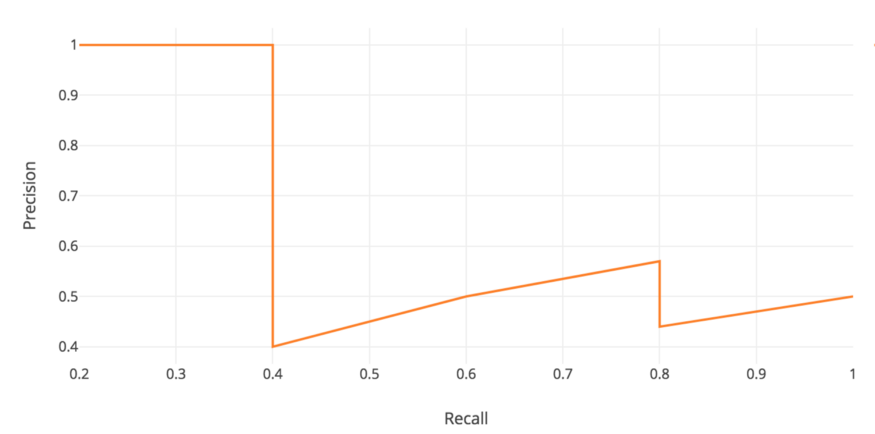
\includegraphics[width=0.7\linewidth]{Images/screensprhot001}
	\caption{Precision-recall curve (Nguồn: \textit{Medium})}
	\label{fig:screensprhot001}
\end{figure}
Định nghĩa tổng quát cho Average Precision (AP) là diện tích phía dưới precision-recall curve 
$$ \text{AP} = \int_{0}^{1}p(r)dr$$
Precision và recall luôn nằm trong đoạn [0; 1] do đó AP cũng nằm trong đoạn [0; 1].  \par
Mean average precision (mAP) là trung bình của AP. Trong một số trường hợp, ta tính AP cho mỗi class và lấy trung bình của chúng, một số khác thì lại giống nhau. Ví dụ theo COCO, không có sự khác biệt giữa AP và mAP.\par
\begin{figure}[!h]
	\centering
	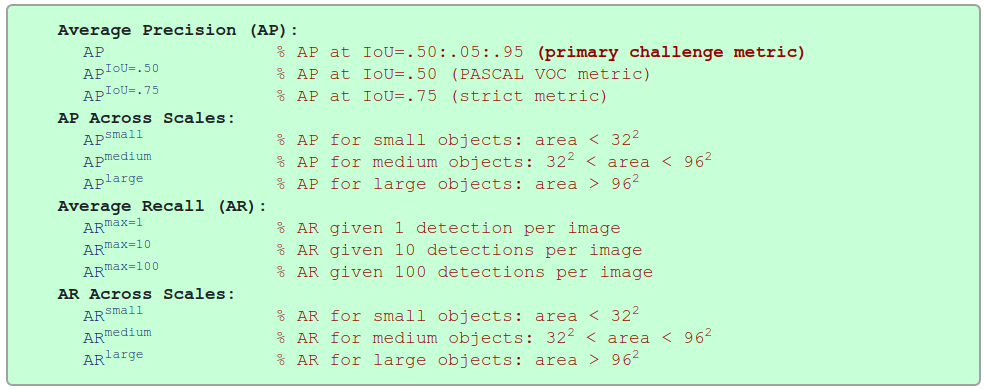
\includegraphics[width=1\linewidth]{Images/cocometric}
	\caption{Một số metric được sử dụng để đánh giá kết quả trên bộ dữ liệu COCO (Nguồn: \textit{cocodataset.org})}
	\label{fig:cocometric}
\end{figure}

\subsection{PyTorch và Faster R-CNN ResNet-50 FPN}
\subsubsection{Sơ lược về Transfer Learning}
Những năm gần đây, Deep Learning phát triển cực nhanh dựa trên lượng dữ liệu training khổng lồ và khả năng tính toán ngày càng được cải tiến của các máy tính. Các kết quả cho bài toán phân loại ảnh ngày càng được nâng cao. Bộ cơ sở dữ liệu thường được dùng nhất là ImageNet với 1.2M ảnh cho 1000 classes khác nhau. Rất nhiều các mô hình Deep Learning đã giành chiến thắng trong các cuộc thi ILSVRC (ImageNet Large Scale Visual Recognition Challenge). Có thể kể ra một vài: AlexNet, ZFNet, GoogLeNet, ResNet, VGG.\par
Nhìn chung, các mô hình này đều bao gồm rất nhiều layers. Các layers phía trước thường là các Convolutional layers kết hợp với các nonlinear activation functions và pooling layers (và được gọi chung là ConvNet). Layer cuối cùng là một Fully Connected Layer và thường là một Softmax Regression (Xem Hình 1). Số lượng units ở layer cuối cùng bằng với số lượng classes (với ImageNet là 1000). Vì vậy output ở layer gần cuối cùng (second to last layer) có thể được coi là feature vectors và Softmax Regression chính là Classifier được sử dụng.\par
Chính nhờ việc features và classifier được trained cùng nhau qua deep networks khiến cho các mô hình này đạt kết quả tốt. Tuy nhiên, những mô hình này đều là các Deep Networks với rất nhiều layers. Việc training dựa trên 1.2M bức ảnh của ImageNet cũng tốn rất nhiều thời gian (2-3 tuần).\par
Với các bài toàn dựa trên tập dữ liệu khác, rất ít khi người ta xây dựng và train lại toàn bộ Network từ đầu, bởi vì có rất ít các cơ sở dữ liệu có kích thước lớn. Thay vào đó, phương pháp thường được dùng là sử dụng các mô hình (nêu phía trên) đã được trained từ trước, và sử dụng một vài kỹ thuật khác để giải quyết bài toán. Phương pháp sử dụng các mô hình có sẵn như thế này được gọi là Transfer Learning.\par
Có 2 loại transfer learning:
\begin{itemize}
	\item \textbf{Feature extractor:} Sau khi lấy ra các đặc điểm của ảnh bằng việc sử dụng ConvNet của pre-trained model, thì ta sẽ dùng linear classifier (linear SVM, softmax classifier,..) để phân loại ảnh.
	\item \textbf{Fine tuning:} Sau khi lấy ra các đặc điểm của ảnh bằng việc sử dụng ConvNet của pre-trained model, thì ta sẽ coi đây là input của 1 CNN mới bằng cách thêm các ConvNet và Fully Connected layer. 
\end{itemize}
\subsection{PyTorch}
PyTorch là một thư viện machine learning mã nguồn mở dựa trên Torch, được sử dụng cho lĩnh vực Thị giác máy tính (Computer Vision) và xử lý ngôn ngữ tự nhiên (Natural language processing), được phát triển bởi Phòng nghiên cứu AI của Facebook (FAIR). Pytorch tập trung vào 2 khả năng chính:
\begin{itemize}
	\item Một sự thay thế cho bộ thư viện numpy để tận dụng sức mạnh tính toán của GPU.
	\item Một platform Deep learning phục vụ trong nghiên cứu, mang lại sự linh hoạt và tốc độ.
\end{itemize}
Cấu trúc dữ liệu cốt lõi được sử dụng trong PyTorch là \textbf{Tensor}.\par
\subsection{Faster R-CNN ResNet-50 FPN}

\textbf{Residual Network (ResNet):} Một vấn đề phổ biến của Deep learning là Vanishing Gradients, tức là theo công thức tính đạo hàm bằng chain rule (trong lan truyền ngược, back propagation), nếu gradient của các lớp sau nhỏ thì gradient ở các lớp đầu sẽ gần bằng 0. Vì thế mà parameter của các lớp trước sẽ không được cập nhật nên các parameter này không đóng góp được gì trong việc đưa ra output. Vậy nên dù ta dùng nhiều lớp, thực chất số lớp hữu ích chỉ là một vài lớp cuối, điều đó làm giảm sự hiệu quả của mạng neural. ResNet ra đời để giải quyết vấn đề đó, giải pháp mà ResNet đưa ra là sử dụng kết nối "tắt" đồng nhất để xuyên qua một hay nhiều lớp. Một khối như vậy được gọi là một Residual Block.\par
\begin{figure}[!h]
	\centering
	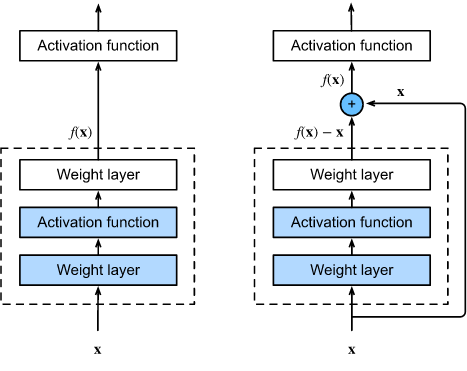
\includegraphics[width=0.5\linewidth]{Images/resnet_1}
	\caption{Khối thường (trái) và khối residual (phải)}
	\label{fig:resnet-1}
\end{figure}
ResNet-50 là một mạng bao gồm 50 lớp residual.\par

\textbf{Mạng kim tự tháp đặc trưng-Feature Pyramid Networks (FPN)} 
Phát hiện các đối tượng có kích thước nhỏ là một vấn đề vô cùng quan
trọng để nâng cao độ chính xác. Và FPN là mô hình mạng được thiết kế
ra dựa trên khái niệm kim tự tháp (pyramid) để giải quyết vấn đề này. \\
\begin{figure}[!h]
	\centering
	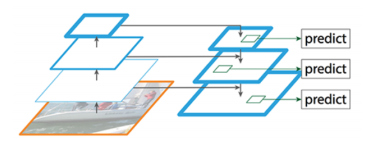
\includegraphics[width=0.5\linewidth]{Images/fpn1}
	\caption{Feature Pyramid Network (FPN)}
	\label{fig:resnet-fpn1}
\end{figure}
\hspace*{1cm}Mô hình FPN giúp nhận diện được cả những đối tượng có kích thước
to và nhỏ nhờ sự kết hợp của tất cả các lớp kim tự tháp. Mô hình được
xây dựng bằng cách thực hiện quá trình bottom-up kết hợp với top-down
để dò tìm đối tượng (trong khi đó, các thuật toán khác chỉ thường sử dụng
bottom-up).Trong đó bottom-up sử dụng mạng tích chập thông thường
dùng để trích xuất các đặc trưng, khi chúng ta ở bottom và đi lên (up) độ
phân giải sẽ giảm, nhưng giá trị cấu trúc cấp cao ( high-level semantic) sẽ
tăng lên. \\
\begin{figure}[!h]
	\centering
	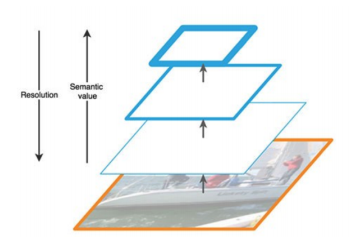
\includegraphics[width=0.5\linewidth]{Images/fpn2}
	\caption{Trích xuất đặc trưng trong mô hình FPN}
	\label{fig:resnet-fpn2}
\end{figure}
%ảnh
Một vài các mô hình khác trong phát hiện đối tượng (ví dụ: SSD,..)
quyết định dựa vào nhiều feature map. Nhưng tầng ở dưới không được
sử dụng để nhận dạng đối tượng. Vì những tầng này có độ phân giải cao
nhưng giá trị cấu trúc cấp cao của chúng lại không đủ cao nên những nhà
nghiên cứu bỏ chúng đi để tăng tốc độ xử lý. Các nhà nghiên cứu biện
minh rằng các tầng ở dưới chưa đủ mức ý nghĩa cần thiết để nâng cao độ
chính xác, thêm các tầng đó vào sẽ không nâng độ chính xác cao thêm bao
nhiêu và họ bỏ chúng đi để có tốc độ tốt hơn. Cho nên, những mô hình phát hiện đối tượng này chỉ sử dụng các tầng ở lớp trên, và do đó sẽ không nhận
dạng được các đối tượng có kích thước nhỏ. \\
\hspace*{1cm}Trong khi đó, FPN xây dựng thêm mô hình top-down, nhằm mục đích
xây dựng các tầng có độ phân giải cao hơn từ các tầng high-level semantics
%ảnh 
\begin{figure}[!h]
	\centering
	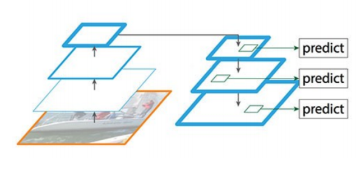
\includegraphics[width=0.5\linewidth]{Images/fpn3}
	\caption{Top-down}
	\label{fig:resnet-fpn3}
\end{figure}
\hspace*{1cm}Trong quá trình xây dựng lại các tầng top-down, chúng ta sẽ gặp một
vấn đề khá nghiêm trọng là bị mất mát thông tin của các đối tượng. Ví dụ
một đối tượng nhỏ khi đi lên (top) sẽ không thấy nó, và từ trên đi ngược
lại sẽ không thể tái tạo lại đối tượng nhỏ đó. Để giải quyết vấn đề này,
chúng ta sẽ tạo các kết nối (skip connection) giữa các reconstruction layer
và các feature maps để giúp quá trình dự đoán các vị trí của đối tượng
thực hiện tốt hơn (sao cho hàm mất mát đạt giá trị nhỏ nhất).  \\
\hspace*{1cm}Đồ hình bên dưới biểu diễn chi tiết đường đi theo bottom-up và topdown. P2, P3, P4, P5 là các pyramid của các feature map. \\
%ảnh
\begin{figure}[!h]
	\centering
	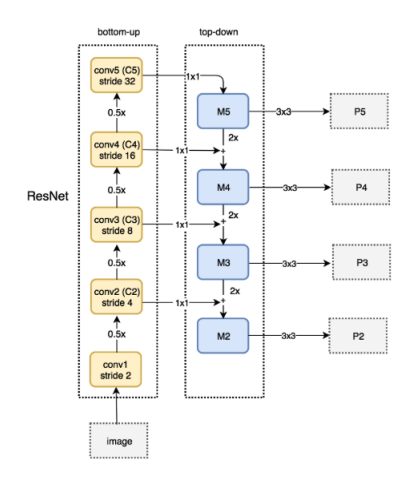
\includegraphics[width=0.5\linewidth]{Images/fpn4}
	\caption{Bottom-up và top-down.}
	\label{fig:resnet-fpn4}
\end{figure}
\hspace*{1cm}FPN không phải là mô hình phát hiện đối tượng. Nó là mô hình phát
hiện đặc trưng và được sử dụng trong phát hiện đối tượng. Các feature
map từ P2 đến P5 trong Hình \ref{fig:resnet-fpn4} độc lập với nhau và các đặc trưng
được sử dụng để phát hiện đối tượng.

\chapter{Ứng dụng học sâu vào bài toán đếm cây trên ảnh viễn thám}
\section{Giới thiệu bài toán}
\hspace*{1cm} Cây keo là một loại cây dễ trồng, có khả năng thích nghi với các loại đất nghèo chất dinh dưỡng, ở những nơi thời tiết khắc nghiệt. Gỗ keo có rất nhiều tác dụng nên keo rất phù hợp với các dự án lâm nghiệp thương mại: là nguyên liệu sử dụng để sản xuất đồ nội thất xuất khẩu và sản xuất giấy. Cây keo ở Việt Nam ngày càng được trồng với quy mô lớn, nhằm nhanh chóng phủ xanh đồi núi trọc keo được trồng thành rừng, đem lại nguồn thu nhập lớn, tạo công ăn việc làm cho nhiều người. Để đáp ứng nhu cầu tiêu thụ gỗ ngày càng tăng ở trong nước và thế giới, sản lượng nông nghiệp tiêu dùng, năng suất cây trồng phải được ước tính. Việc phát hiện, kiểm soát cây keo trên một diện tích lớn trong khu rừng giúp cho doanh nghiệp và các nhà quản lý biết được tình trạng hiện tại của các cây keo, có thể trồng thêm được cây nào vào những khu đất còn trống. Tuy nhiên việc thu thập thủ công dữ liệu cây trồng để lưu trữ hồ sơ trên một diện tích đất lớn là không khả thi đối với con người, gây tốn kém tiền bạc và dễ bị ảnh hưởng bởi lỗi của con người. \\
\hspace*{1cm} Một tiềm năng lớn để giải quyết vấn đề này là sử dụng các hình ảnh vệ tinh
kết hợp với các thuật toán thị giác máy tính để phát hiện quản lý những cây trồng này. Sử dụng hình ảnh vệ tinh để khảo sát sẽ giảm bớt một phần công việc của con người khi phải trực tiếp đến khu vực đó tiến hành theo dõi, phân tích. Các bức ảnh viễn thãm được chụp lại với kích thước lớn, có thể bao quát một khu diện tích đất trồng rộng giúp tiết kiệm thời gian điều tra khảo sát, từ đó giúp các nhà quản lý của doanh nghiệp có thể nắm bắt tình hình kịp thời, lập kệ hoạch sản xuất phù hợp \\
\hspace*{1cm}Để việc giải quyết bài toán này trở nên đơn giản và tự động hơn, trong Đồ án
này, em trình bày về việc sử dụng các phương pháp Deep Learning để tiến hành phân
tích.


\section{Mô hình hoá bài toán và thiết kế dữ liệu luyện}
\begin{enumerate}[label= \textit{\alph*)}]
\item \textit{Mô hình hóa bài toán} \\
\textbf{Input:} \\
Ảnh viễn thám được lưu ở định dạng .tif, có kích thước lớn (từ vài chục MB đến GB) \\ \textbf{Tiền xử lý:} \\
Ảnh đầu vào sẽ được chia nhỏ thành các ảnh có kích thước $256 \times 256$ (bằng với kích thước trong tập ảnh training),  với tỉ lệ \textit{overlap} giữa các tấm ảnh là $0.5$ \\
\textbf{Output:} \\
Các file định dạng txt chứa các bounding box mà mô hình đoán đó là vật thể trong bức ảnh đó.  
Vì mục tiêu của bài toán là nhận dạng và đếm số cây trên một bức ảnh lớn,  nên ta sẽ ghép các tấm ảnh nhỏ ở trên lại để đưa về hình ảnh gốc của chúng.  Vì trong quá trình tiền xử lý, ta thiết lập overlap $= 0.5$ nên việc các bounding box của các bức ảnh gần nhau sẽ đè lên nhau,  gây ra hiện tượng trùng lặp.  Để giải quyết vấn đề này,  các bounding box thu được trên toàn bộ các ảnh đầu tiên sẽ được đưa về toạ độ địa lý, sau đó sử dụng thuật toán NMS để loại bỏ các bounding box trùng nhau (nếu như giá trị IOU của hai bounding box này vượt quá một ngưỡng (trong mô hình này em lấy ngưỡng $=0.3$)).  Kết quả sau khi thực hiện thuật toán NMS sẽ 


\item \textit{Thiết kế dữ liệu luyện mạng} \\
Dữ liệu sử dụng trong bài toán này được cung cấp bởi thầy giáo hướng dẫn TS.  Lê Hải Hà.  Dữ liệu bao gồm 2 thư mục,  nỗi thư mực gồm một vài ảnh ở định dạng GeoTif và các \textbf{shapefile} chưa toạ độ các bounding box trong các bức ảnh đó
 \begin{figure}[!htb]
	\centering
	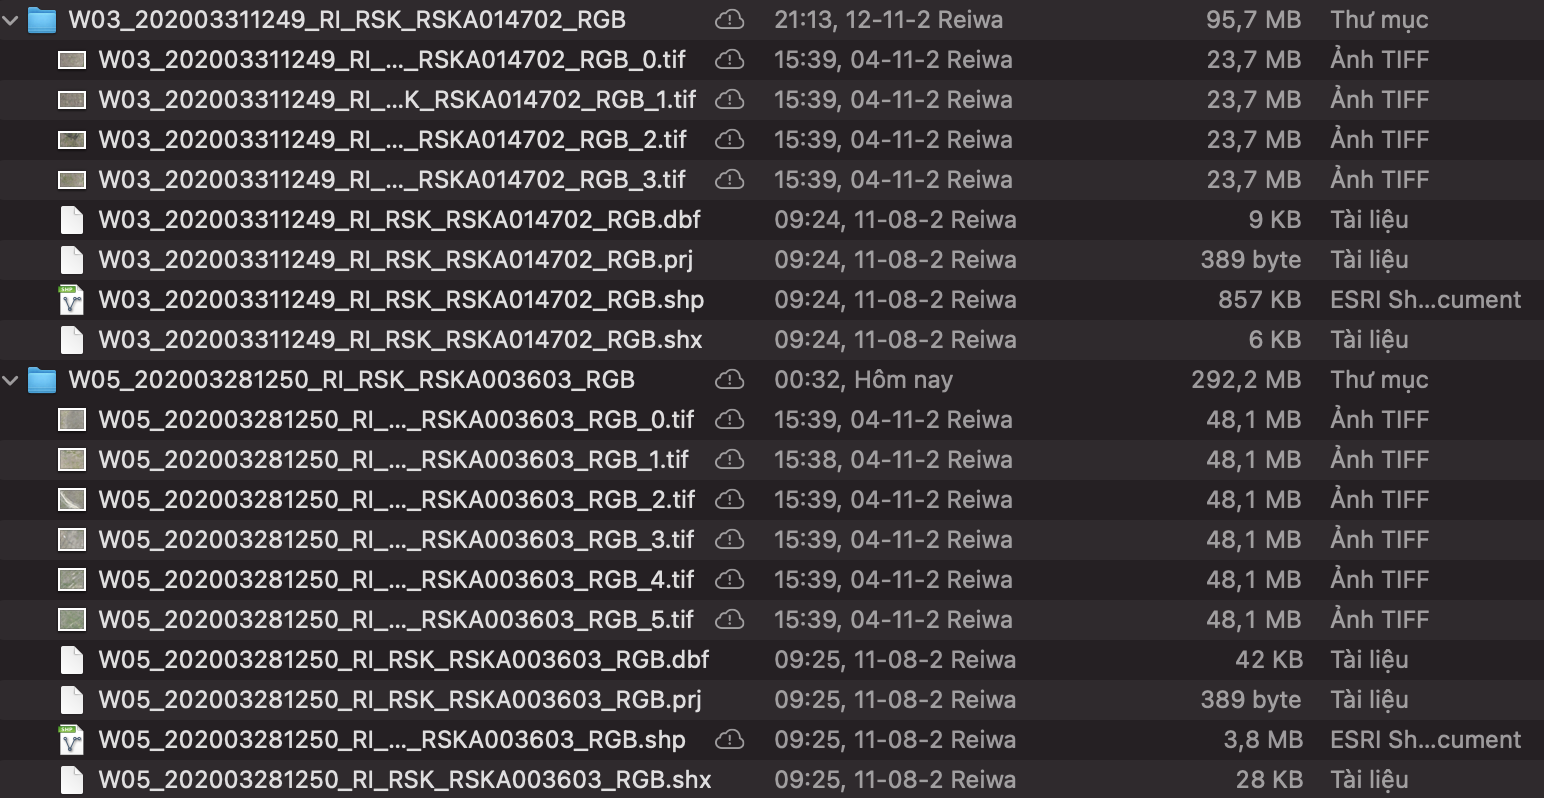
\includegraphics[width=1\linewidth]{Images/data_folder}
	\caption{Dữ liệu sử dụng trong bài toán}
	\label{fig:data_folder}
\end{figure}

\newpage
 \begin{figure}[!htb]
	\centering
	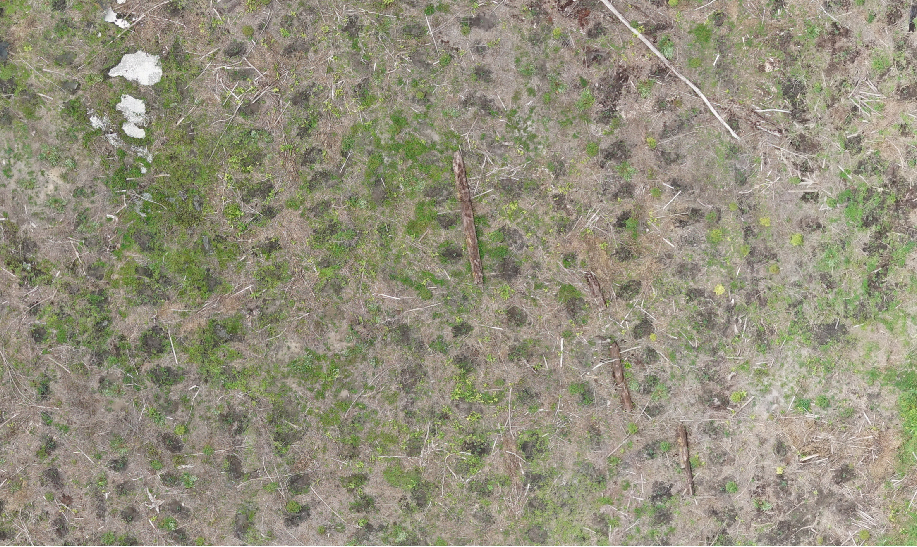
\includegraphics[width=1\linewidth]{Images/qgisa}
	\caption{Minh hoạ ảnh viễn thám với phần mềm QGIS} 
	\label{fig:1a}
\end{figure}


 \begin{figure}[!htb]
	\centering
	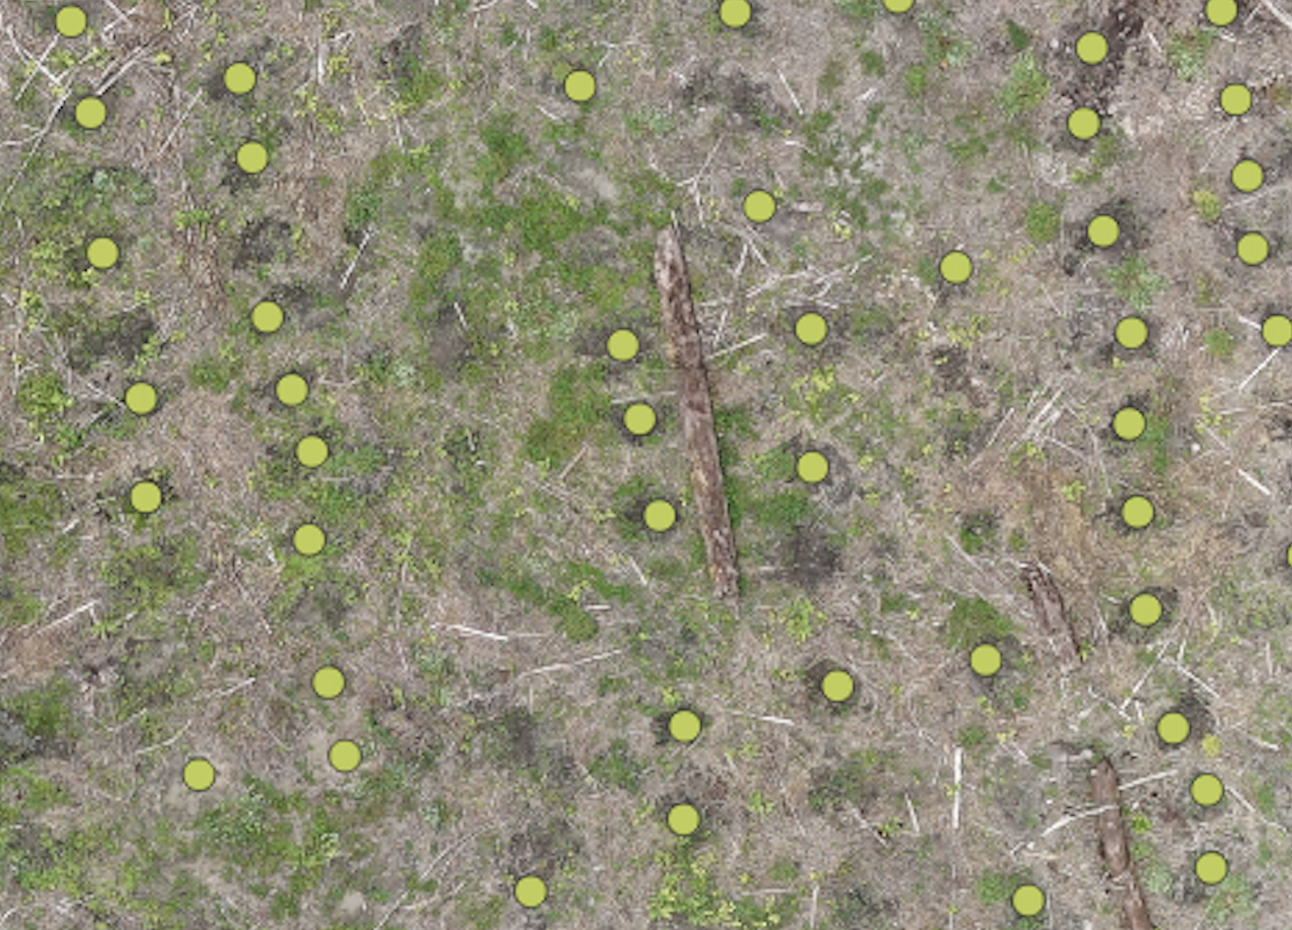
\includegraphics[width=0.7\linewidth]{Images/qgisb}
	\caption{Toạ độ các bounding box trên ảnh,  biểu thị bởi các hình tròn màu vàng}
	\label{fig:1b}
\end{figure}


%\begin{figure}
%  \begin{subfigure}{0.6\textwidth}
%    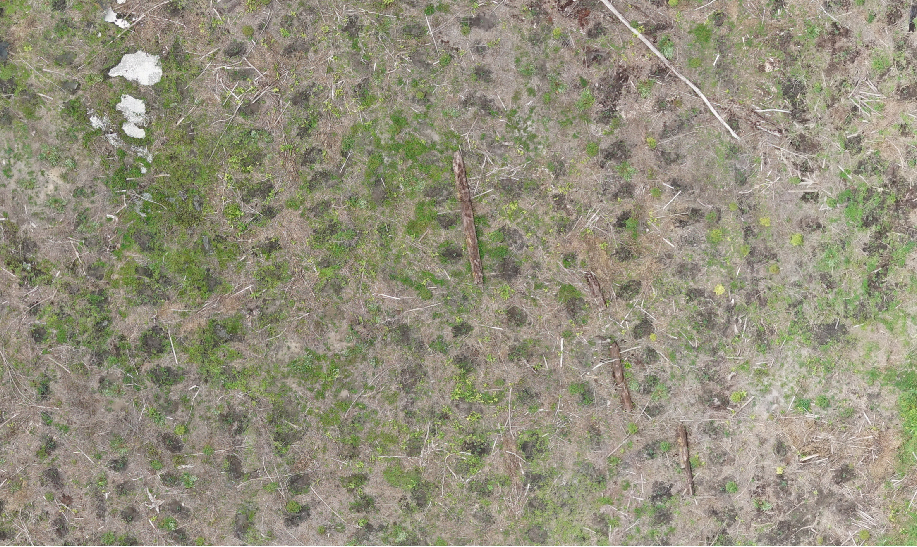
\includegraphics[width=\linewidth]{Images/qgisa}
%    \caption{} \label{fig:1a}
%  \end{subfigure}%
%  \hspace*{\fill}   % maximize separation between the subfigures
%  \begin{subfigure}{0.5\textwidth}
%    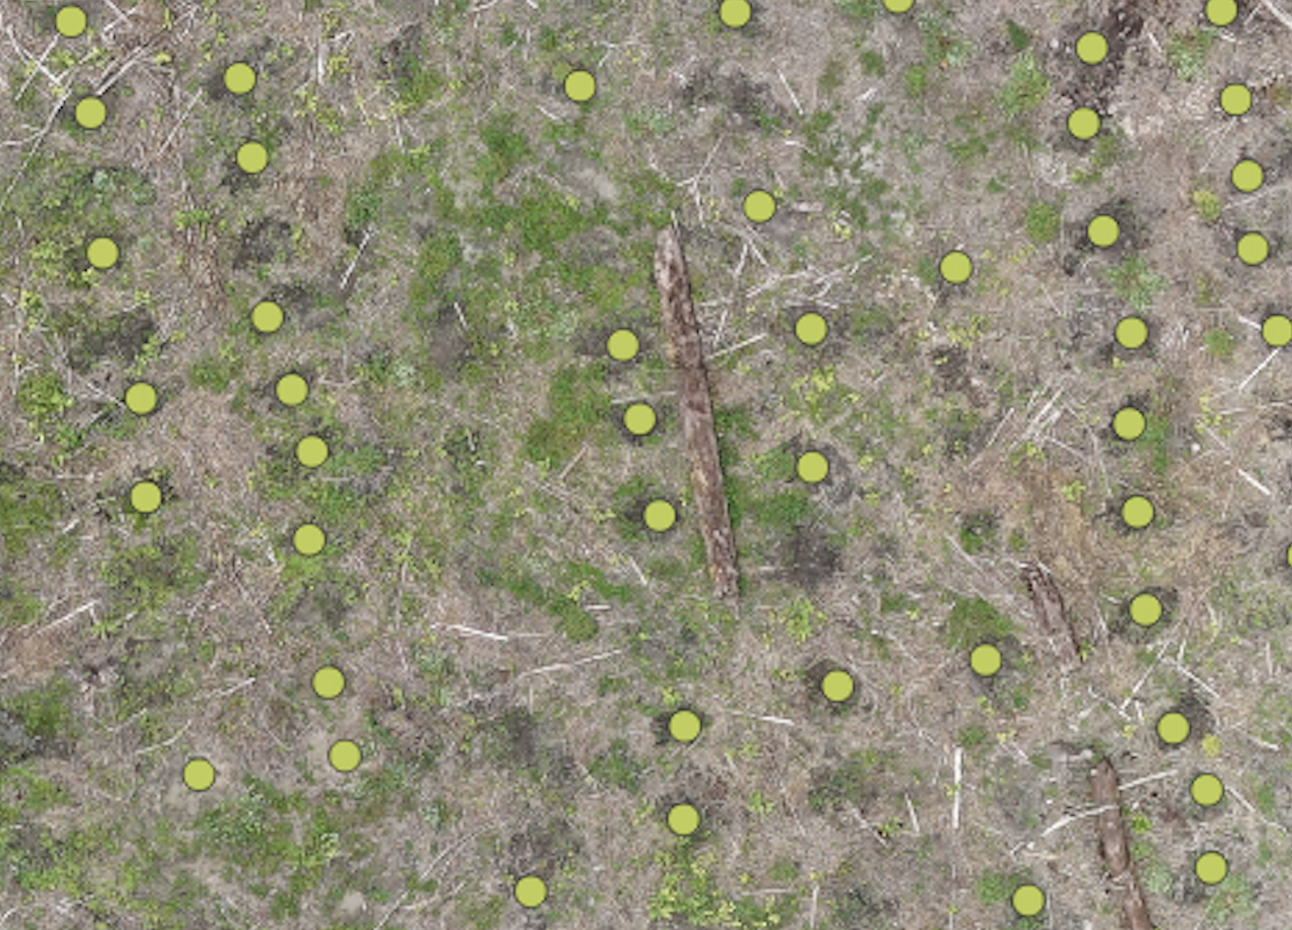
\includegraphics[width=\linewidth]{Images/qgisb}
%    \caption{} \label{fig:1b}
%  \end{subfigure}%
%  \hspace*{\fill}   % maximizeseparation between the subfigures

%
%\caption{Minh hoạ ảnh viễn thám với phần mềm QGIS (hình \ref{fig:1a}),  toạ độ các bounding box trên ảnh,  biểu thị bởi các hình tròn màu vàng (hình \ref{fig:1b})} \label{fig:1}
%\end{figure}
\newpage
Các ảnh trong bộ dữ liệu ở trên có 2 loại kích thước : $3141 \times 1885$ và $3874 \times 3100$.  Để thuận tiện cho việc training mô hình,  ta sẽ chia nhỏ mỗi ảnh thành nhiều ảnh con có kích thước $256 \times 256$ với giá trị $overlap = 0.5$.  Để lấy bounding box trong từng bức ảnh được cắt ra,  đầu tiên ta tiến hành đọc file \textit{shapefile} của ảnh đó bằng thư viện \textit{geopandas} (hình \ref{fig:polygon_ori}): 

 \begin{figure}[!h]
	\centering
	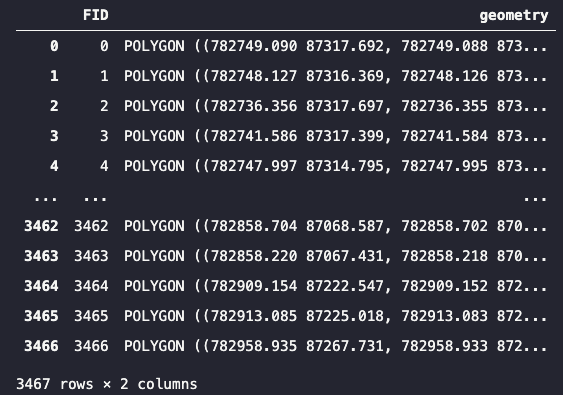
\includegraphics[width=1\linewidth]{Images/polygon_ori}
	\caption{Đọc file shapefile với thư viện geopandas}
	\label{fig:polygon_ori}
\end{figure}
Vì toạ độ các câu được đánh dấu theo hình tròn nên ta cần chuyển định dạng hình tròn về bounding box (hình \ref{fig:polygon_bounds})

 \begin{figure}[!h]
	\centering
	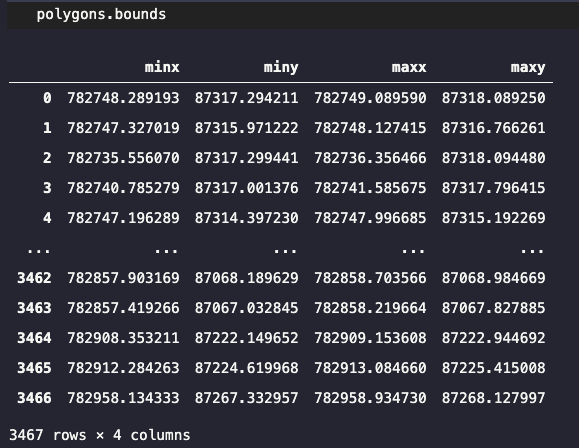
\includegraphics[width=1\linewidth]{Images/polygon_bounds}
	\caption{Toạ độ 4 đỉnh của một polygon}
	\label{fig:polygon_bounds}
\end{figure}


%\begin{figure}
%  \begin{subfigure}{0.5\textwidth}
%    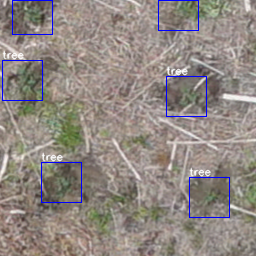
\includegraphics[width=\linewidth]{Images/split1}
%    \caption{} \label{fig:1a}
%  \end{subfigure}%
%  \hspace*{\fill}   % maximize separation between the subfigures
%  \begin{subfigure}{0.5\textwidth}
%    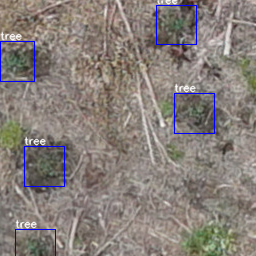
\includegraphics[width=\linewidth]{Images/split2}
%    \caption{} \label{fig:1b}
%  \end{subfigure}%
%  \hspace*{\fill}   % maximizeseparation between the subfigures
%%    \begin{subfigure}{0.4\textwidth}
%%    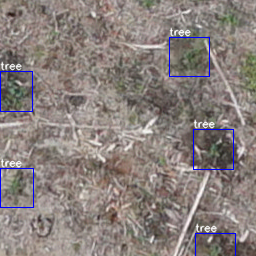
\includegraphics[width=\linewidth]{Images/split3}
%%    \caption{} \label{fig:1b}
%%  \end{subfigure}%
%\caption{Minh hoạ ảnh viễn thám với phần mềm QGIS (hình \ref{fig:1a}),  toạ độ các bounding box trên ảnh,  biểu thị bởi các hình tròn màu vàng (hình \ref{fig:1b})} \label{fig:1}
%\end{figure}
%
% \begin{figure}[!h]
%	\centering
%	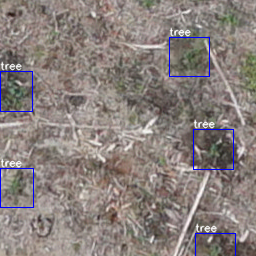
\includegraphics[width=0.5\linewidth]{Images/split3}
%	\caption{Toạ độ 4 đỉnh của một polygon}
%	\label{fig:polygon_bounds}
%\end{figure}
\newpage
Tuy nhiên trong hình trên, mỗi điểm là một toạ độ trên một mặt phẳng địa lý,  ta phải chuyển các toạ độ $x,y$ về toạ độ cột,  hàng tương ứng.  Một vài kết quả thu được sau khi tiến hành cắt ảnh và lấy bounding box tương ứng cho mỗi bức ảnh đó: 
\newpage
\begin{figure}[!h]
    \centering
    \begin{subfigure}[!h]{0.45\textwidth}
    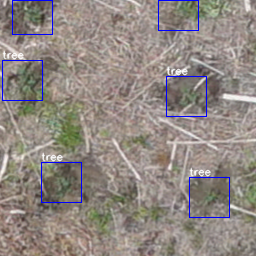
\includegraphics[width=\linewidth]{Images/split1}
        \subcaption[short for lof]{}
%        \rule{\linewidth}{3cm}
        \label{fig:subfig1}
    \end{subfigure}%
    \quad
    \begin{subfigure}[!h]{0.45\textwidth}
    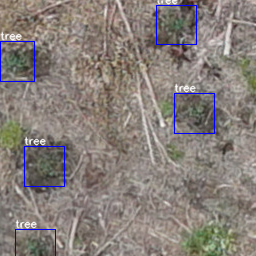
\includegraphics[width=\linewidth]{Images/split2}
        \subcaption[short for lof]{}
%        \rule{\linewidth}{3cm}
        \label{fig:subfig2}
    \end{subfigure}
 
    \begin{subfigure}[!h]{0.45\textwidth}
    	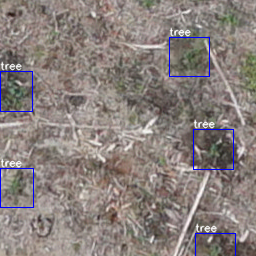
\includegraphics[width=\linewidth]{Images/split3}
        \subcaption[short for lof]{}
%        \rule{\linewidth}{3cm}
        \label{fig:subfig3}
    \end{subfigure}
    \caption[Optional caption for list of figures]{Main caption for subfigures \subref{fig:subfig1}, \subref{fig:subfig2} and \subref{fig:subfig3}}
\end{figure}
\end{enumerate}
Kết quả sau khi cắt ảnh ra ta thu được bộ dữ liệu hơn 5000 ảnh kích thước $256 \times 256$ cùng với toạ độ các bounding box tương ứng trong từng ảnh đó
\section{Huấn luyện mạng neural}
Chúng ta sẽ tiến hành huấn luyện mô hình dựa trên bộ dữ liệu được tạo ra ở trên.  Mô hình mà em sử dụng trong bài toán này là Faster- RCNN; trong đó backbone sử dụng ở đây là ResNet101 phục vụ cho việc trích xuất các đặc trưng trong ảnh
\section{Xây dựng chương trình}

\chapter{Cài đặt chương trình và đánh giá kết quả}

\section{Môi trường cài đặt chương trình và các yêu cầu liên quan}
\subsection{Môi trường cài đặt chương trình}
Chương trình được cài đặt trên ngôn ngữ Python (phiên bản 3.6.9) và được thử nghiệm trên hệ điều hành máy ảo của google colab sử dụng chip 4 cores , bộ nhớ RAM 24GB,  card đồ hoạ NVIDIA Tesla V100 16GB (hình \ref{fig:nvidia-smi})
 \begin{figure}[!h]
	\centering
	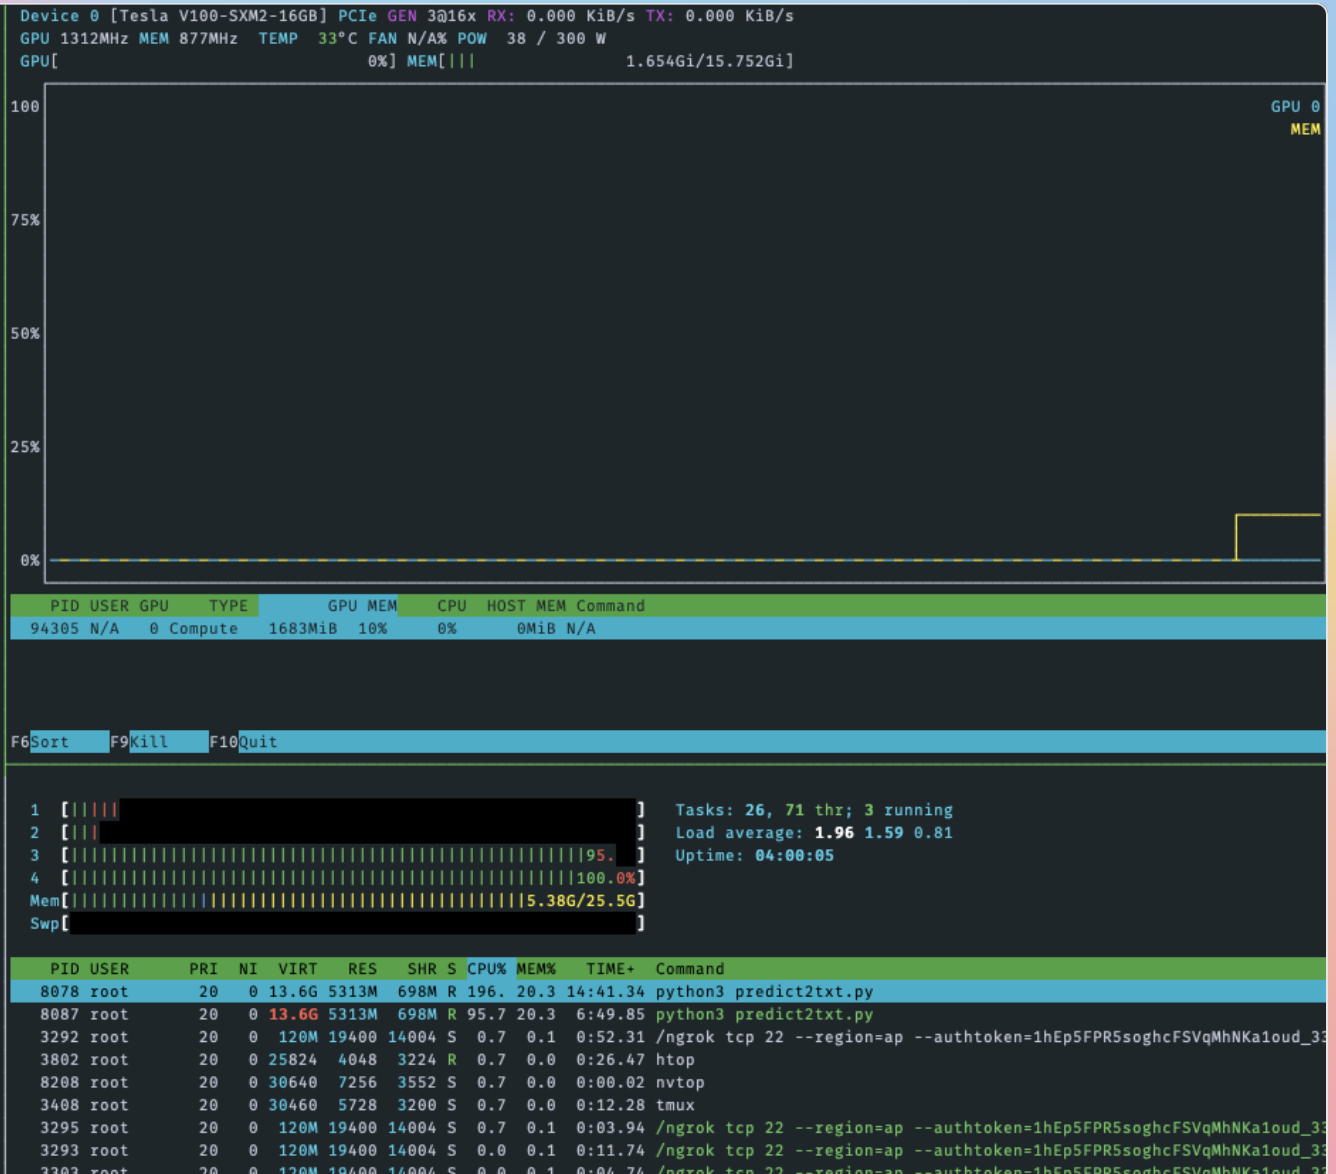
\includegraphics[width=0.8\linewidth]{Images/nvidia-smi}
	\caption{Cấu hình máy tính sử dụng cho bài toán}
	\label{fig:nvidia-smi}
\end{figure}
\subsection{Các yêu cầu liên quan}
\begin{itemize}
	\item Ngôn ngữ sử dụng: Python phiên bản 3.6.9
	\item IDE sử dụng: Visual Studio Code
	\item Các thư viện Python sử dụng: pandas, numpy, matplotlib,  torch, os , cv2 và xlwt.
\end{itemize}



\section{Dữ liệu đầu vào}
Vì dữ liệu em được cung cấp bị hạn chế, nên trong bộ dữ liệu ban đầu em lấy ra 1 ảnh chưa được xử lý cho tập train và validation (hình \ref{fig:demo}) để làm dữ liệu đầu vào cho mô hình nhận diện vật thể đã xây dựng ở chương trước.  Lý do của việc lấy một ảnh kích thước lớn để dự đoán là vì theo yêu cầu của khách hàng,  họ cần đánh giá kết quả mô hình trên toàn bộ diện tích đất của họ chứ không phải các tấm ảnh kích thước $256 \times 256$ được cắt nhỏ từ tấm ảnh ban đầu
 \begin{figure}[!h]
	\centering
	\includegraphics[width=1\linewidth]{Images/demo}
	\caption{Dữ liệu đầu vào để phát hiện vật thể}
	\label{fig:demo}
\end{figure}

\section{Kết quả mô hình}
Thời gian chạy chương trình cho ảnh trên: $43$ giây \\
Hình ảnh kết quả được lưu lại ở dạng shapefile: 	(hình \ref{fig:shpfile_demo_result})
 \begin{figure}[!h]
	\centering
	\includegraphics[width=0.5\linewidth]{Images/shpfile_demo_result}
	\caption{Kết quả mô hình: thư mục chứa các shapfile}
	\label{fig:shpfile_demo_result}
\end{figure}




Ta sử dụng file shapefile ở trên để mô phỏng kết quả trên phần mềm QGIS (hình \ref{fig:demo_result}): 
 \begin{figure}[!h]
	\centering
	\includegraphics[width=1\linewidth]{Images/demo_result}
	\caption{Kết quả mô hình: các ô vuông màu xanh là kết quả phát hiện của mô hình; chấm màu cam là các cây được gán nhãn sẵn. }
	\label{fig:demo_result}
\end{figure}


\section{Đánh giá kết quả}
Hình \ref{fig:demo_result} ở trên chỉ cho ta một cách khái quát về kết quả mô hình khi so sánh với các bounding box ban đầu.  Để đánh giá kết quả của mô hình,  trước tiên ta định nghĩa 2 bounding box cùng phát hiện một đối tượng nếu giá trị IOU của chúng $\geq 0.3$. Khi đó,  bounding box được dự đoán từ mô hình sẽ được coi là một \textit{True positive},  ngược lại sẽ là \textit{False positive}.  Trong trường hợp có nhiều hơn 1 bounding box cùng dự đoán một đối tượng,  ta sẽ lấy bounding box có confidence (độ tin cậy) cao nhất làm TP, các bounding box còn lại sẽ là FP.  Để so sánh một cách khách quan, em sử dụng cùng một tập các thang đo phổ biến là Precision, Recall và F1-score.  Trong đó, Precision là tỉ lệ giữa số tên miền phân loại chính xác trên tổng số tên miền được dự đoán của mỗi lớp. Recall là tỉ lệ giữa số tên miền được
phân loại đúng theo một nhãn trên tổng số tên miền được gán theo nhãn đó.
F1-score là trung bình điều hòa giữa hai giá trị Precision và Recall. Các tham
số trên được biểu diễn trong các biểu thức:
\begin{equation*}
	Precision = \frac{TP}{TP + FP}
\end{equation*}

\begin{equation*}
	Recall = \frac{TP}{TP + FN}
\end{equation*}

\begin{equation*}
	F1 - score = \frac{2 \times Precision \times Recall}{Precision + Recall}
\end{equation*}
%Lần lượt tính toán các bounding box và áp dụng công thức của Precision,  Recall,  F1,  ta thu được các thông số cho việc đánh giá kết quả như sau: 
\begin{figure}[!h]
	\centering
  	\includegraphics[width=.8\linewidth]{Images/f1-score} %example-image-a
 	 \caption{Đánh giá kết quả}
 	 \label{fig:sub1}
\end{figure}

\section{Định hướng phát triển trong tương lai}
Từ kết quả thực nghiệm cho thấy, chương trình đã có những thành công nhất định. Song bên cạnh đó cũng còn khá nhiều nhược điểm cần cải tiến. Trong quá trình hoàn thành đồ án em đã đầu tư nhiều thời gian và công sức với bài toán này, và nhận thấy đây là bài toán có khả năng phát triển cao hơn nữa . Em xin đưa ra một số hướng phát triển tiếp theo cho bài toán như sau:
\begin{itemize}
	\item Phát triển và cài đặt giao diện chương trình để có thể dễ dàng chạy và sử dụng hơn. 
	\item Sử dụng thêm một vài phép xử lý ảnh để tăng cường dữ liệu phục vụ cho việc training 
	\item Cải tiến, thay đổi các thuật toán để loại bỏ các bounding box trùng nhau nhanh hơn khi sử dụng thuật toán NMS; giúp chương trình chạy tối ưu hơn
\end{itemize}




%\begin{figure}
%\centering
%\begin{subfigure}{.5\textwidth}
%  \centering
%  \includegraphics[width=.4\linewidth]{example-image-a}
%  \caption{A subfigure}
%  \label{fig:sub1}
%\end{subfigure}%
%\begin{subfigure}{.5\textwidth}
%  \centering
%  \includegraphics[width=.4\linewidth]{example-image-a}
%  \caption{A subfigure}
%  \label{fig:sub2}
%\end{subfigure}
%\caption{A figure with two subfigures}
%\label{fig:test}
%\end{figure}

\chapter*{Tài liệu tham khảo}
\addcontentsline{toc}{chapter}{Tài liệu tham khảo}
\mdseries 
\textbf{Tài liệu tham khảo tiếng Việt}

\begin{enumerate}[label=\textrm{[\arabic*.]}]
\item Nguyễn Đức Nghĩa, Nguyễn Tô Thành, "Toán rời rạc", Nhà xuất bản Đại Học Quốc Gia Hà Nội, 1997, tr. 147-155.
\item Tống Đình Quỳ, "Giáo trình xác suất thống kê", Nhà xuất bản Bách Khoa-Hà Nội, 2016.
\end{enumerate}
 \textbf{Tài liệu tham khảo tiếng Anh}
\begin{enumerate}[label=\textrm{[\arabic*.]}]
\item
	Martin Aigner, Günter M. Ziegler, ‘‘Proofs from THE BOOK’’, $6^{th}$ Edition.
\item
	Valle Martinez, Vicente, "Notes on the proof of the van der Waerden permanent conjecture" (2018).
\end{enumerate}





\end{document}